\documentclass[final,onefignum]{siamart190516}
%\documentclass[review,onefignum]{siamart190516}

\usepackage{amssymb,bbm}
\usepackage{pgfplots,tikz}
\pgfplotsset{compat=1.14}

\newtheorem{example}{Example}

% math macros
\newcommand\bb{\mathbf{b}}
\newcommand\bbf{\mathbf{f}}
\newcommand\bg{\mathbf{g}}
\newcommand\bn{\mathbf{n}}
\newcommand\bq{\mathbf{q}}
\newcommand\br{\mathbf{r}}
\newcommand\bu{\mathbf{u}}
\newcommand\bv{\mathbf{v}}
\newcommand\bx{\mathbf{x}}
\newcommand\by{\mathbf{y}}

\newcommand\bG{\mathbf{G}}
\newcommand\bQ{\mathbf{Q}}
\newcommand\bV{\mathbf{V}}
\newcommand\bX{\mathbf{X}}
\newcommand\bY{\mathbf{Y}}

\newcommand\CC{\mathbb{C}}
\newcommand{\DDt}[1]{\ensuremath{\frac{d #1}{d t}}}
\newcommand{\ddt}[1]{\ensuremath{\frac{\partial #1}{\partial t}}}
\newcommand{\ddx}[1]{\ensuremath{\frac{\partial #1}{\partial x}}}
\newcommand{\ddy}[1]{\ensuremath{\frac{\partial #1}{\partial y}}}
\newcommand{\ddxp}[1]{\ensuremath{\frac{\partial #1}{\partial x'}}}
\newcommand{\ddz}[1]{\ensuremath{\frac{\partial #1}{\partial z}}}
\newcommand{\ddxx}[1]{\ensuremath{\frac{\partial^2 #1}{\partial x^2}}}
\newcommand{\ddyy}[1]{\ensuremath{\frac{\partial^2 #1}{\partial y^2}}}
\newcommand{\ddxy}[1]{\ensuremath{\frac{\partial^2 #1}{\partial x \partial y}}}
\newcommand{\ddzz}[1]{\ensuremath{\frac{\partial^2 #1}{\partial z^2}}}
\newcommand{\Div}{\nabla\cdot}
\newcommand\eps{\epsilon}
\newcommand{\grad}{\nabla}
\newcommand{\ihat}{\mathbf{i}}
\newcommand{\ip}[2]{\ensuremath{\left<#1,#2\right>}}
\newcommand{\jhat}{\mathbf{j}}
\newcommand{\khat}{\mathbf{k}}
\newcommand{\nhat}{\mathbf{n}}
\newcommand\lam{\lambda}
\newcommand\lap{\triangle}
\newcommand\Matlab{\textsc{Matlab}\xspace}
\newcommand\RR{\mathbb{R}}
\newcommand\vf{\varphi}



\title{Conservation laws for free-boundary fluid layers\thanks{Draft date: \today.  Supported by NASA grant \# NNX13AM16G.}}

\author{Ed Bueler\thanks{Dept.~of Mathematics and Statistics, University of Alaska Fairbanks \,\, (\texttt{elbueler@alaska.edu}).}}

\begin{document}
\maketitle

\begin{abstract}
Time-dependent models of fluid motion in thin layers, subject to signed source terms, represent important sub-problems within climate dynamics.  Examples include ice sheets, sea ice, and even shallow oceans and lakes.  We address these problems as discrete-time sequences of continuous-space weak formulations, namely (monotone) variational inequalities or complementarity problems, in which the conserved quantity is the layer thickness.  Free boundaries wherein the thickness and mass flux both go to zero at the margin of the fluid layer generically arise in such models.  After showing these problems are well-posed in several cases, we consider the limitations to discrete conservation in numerical schemes.  A free boundary in a region of negative source---an ablation-caused margin---turns out to be a barrier to exact conservation in either a continuous- or discrete-space sense.  We then propose computable \emph{a posteriori} quantities which allow conservation-error bounds in finite volume and finite element schemes.
\end{abstract}


\pagestyle{myheadings}
\thispagestyle{plain}
\markboth{ED BUELER}{CONSERVATION LAWS FOR FREE-BOUNDARY FLUID LAYERS}


\section{Introduction}  \label{sec:intro}

Consider a thin layer of fluid which is free to move about on a solid substrate.  Suppose that, in addition, mass can be added (accumulation, precipitation) or removed (ablation, evaporation) from the fluid layer by external processes.  Through flow and these addition/removal processes, the geometry of the layer varies in time and space.  We consider models of such fluid layers in which the layer geometry is described by a nonnegative thickness function.  In such models the addition/removal processes can be combined into a signed source term in a two-spatial-dimension mass conservation (or balance) equation.  Note that the addition/removal processes and the substrate topography are defined on a larger (fixed) region than the fluid-covered area.  Assuming the thickness function is continuous, the conservation equation applies only in the open set where the thickness is positive.  The problem of simultaneously determining the fluid motion and the fluid-covered domain is of free-boundary type.

The physics of such models couples the mass conservation equation to additional momentum and energy conservation laws.  The addition/removal processes, i.e.~the ``climate'' of the fluid layer, may also be coupled to the conservation equations, as when glacier thickness affects surface elevation and thus the precipitation rate.  Solving the resulting model, combining conservation equations, addition/removal processes, and additional closure relationships as needed, determines the nontrivial manner in which the layer geometry evolves.

This paper contains a basic, necessarily incomplete, analysis of the mathematical well-posedness of such climate-driven fluid layer models.  We start by extracting the minimal mathematical form, namely a scalar conservation equation and the nonnegative-thickness constraint.  After considering well-posedness based on several flux-form possibilities, we address tradeoffs and barriers inherent in the numerical solutions of such models.

Problems of this type appear within models of glaciers and ice sheets \cite{Bueler2016,CalvoDuranyVazquez2000,DiazSchiavi1999,
EgholmNielsen2010,JouvetBueler2012,JouvetBuelerGraeserKornhuber2013}, surface and subsurface hydrology \cite{AlonsoSantillanaDawson2008,Maxwelletal2015}, and sea ice \cite{LipscombHunke2004,Thorndikeetal1975}.  Generally, multiphysics Earth system models often contain thin-layer, free-boundary sub-models for various species (or phases) of fluids.  For example, in comprehensive models of glaciers and ice sheets there are submodels describing supra- and subglacial hydrology of liquid water \cite{Aschwandenetal2012,BuelervanPelt2015,Schoofetal2012}, floating ice shelves \cite{Albrechtetal2011}, and sediment transport \cite{Brinkerhoffetal2017}.

In such geophysical and climate-modeling contexts, determining the fluid-covered area is a leading-order modeling goal.  For example, snow and ice are much more reflective than the substrate they cover (i.e.~land or ocean), so deciding whether grid cells are ice-covered or ice-free is a significant modeling purpose.  A goal of equal importance is the conservation of mass, including a precise accounting of mass transfers to and from the modeled fluid phases.

The above geophysical applications drive the author's interest, but the situation is as familiar as the dynamics of rain droplets on a car windshield.  Precipitation, evaporation, gravity, wind stresses, and surface tension all combine to determine the evolution of the geometry of the drops and rivulets, and of the wetted and dry domains.  Note that models of such thin fluid flows often have not included any source term \cite[for example]{Kondic2003}, but those that include evaporation will require active enforcement of nonnegative layer thickness.

If the fluid is modeled as having constant density then the (nonnegative) layer thickness can be regarded as the conserved quantity, equivalent to mass per unit area.  In models for variable density fluids the vertical integral of density is the conserved quantity (in the two-dimensional conservation equation) and this variable must also be nonnegative.  For simplicity we consider the constant-density case and we call the conserved quantity ``mass'' and the corresponding nonnegative variable ``thickness''.

Now, to be more precise let us suppose that $\Omega \subset \RR^d$ is a bounded open region with regular (Lipschitz) boundary; note $d=1,2$ in cases of geophysical interest.  The layer thickness function $u(x,t)$ is defined for $x\in \Omega$ and $t \in [0,T]$.  Where there is no fluid we have $u(x,t)=0$.  The rate of flow is described by a vector flux $\bq$ and the climate (i.e.~the addition/removal processes) by a scalar, signed source term $f$; we discuss parameterizations below.

The models we consider are usually stated in strong form.  They include at least a mass conservation equation and an obvious, though sometimes-unstated, inequality constraint:
\begin{align}
u_t + \Div \bq &= f &&\text{in } \Omega \times (0,T), \text{ where } u > 0 \label{eq:massconserve} \\
u &\ge 0 &&\text{in } \Omega \times [0,T], \label{eq:constraint}
\end{align}
along with an initial condition $u(x,0)=u_0(x)\ge 0$ defined on $\Omega$.  We emphasize that conservation equation \eqref{eq:massconserve} applies only where the fluid is present ($u>0$), and not in the remainder of $\Omega$.  The situation is pictured in Figure \ref{fig:cartoon}, where positive source values ($f>0$) are pictured as downward arrows (precipitation).

\begin{figure}[ht]
\centerline{\includegraphics[width=0.8\textwidth]{figs/cartoon}}
\caption{Schematic of a fluid layer with a thickness $u\ge 0$.}
\label{fig:cartoon}
\end{figure}

Evidently, analyzing the well-posedness of any model including \eqref{eq:massconserve} and \eqref{eq:constraint} requires additional information about $\bq$ and $f$, along with a specification of a space of admissible solutions $u$.  In most of this article we suppose that the flux $\bq$ is local, but otherwise quite general:
\begin{equation}
\bq = \bq(\grad u(x,t),u(x,t),x,t). \label{eq:fluxdepends}
\end{equation}
However, Subsection \ref{subsec:nonlocal} considers models where $\bq$ depends non-locally on integrals of $u$ over $\Omega$.  In many realistic models, computing this non-local dependence involves solving coupled differential equations.

In \eqref{eq:fluxdepends}, dependence of the flux on thickness is to be expected---thicker layers move more mass---as is dependence on $x$ because of substrate variations \cite[for example]{Bueler2016}.  The flux may additionally depend on $\grad u$ in flows which are gravity-driven and viscous; such flows are at least partly diffusive.  In simple cases the flux might be written in the form $\bq=- D \grad u + \bq_a$ where $D > 0$ has various dependence on $t,x,u,|\grad u|$---see Subsections \ref{subsec:plap} and \ref{subsec:powertransform} below---with the advective flux $\bq_a$ perhaps independent of $\grad u$.  In fact, equation \eqref{eq:massconserve} may be dominantly advective.  In the simplest advective case mass moves at some vertically-averaged velocity $\bX=\bX(x,t)$ determined by external factors, and we then have $\bq_a = \bX u$; see Subsection \ref{subsec:advect}.  In such cases we will add a small diffusion term to establish well-posedness.  Our results for such advective fluxes will apply even if $\bX$ comes from a (coupled) solution of a momentum conservation system, for example, as long as it has the regularity needed to apply the theory (Subsection \ref{subsec:fluxassumptions}).

In \eqref{eq:massconserve} the source function $f$ is allowed to be nonlinear in $u$ because feedback between layer thickness $u$ and the source $f$ occurs in certain applications \cite{Jouvetetal2011}.  However, when proving well-posedness in Section \ref{sec:wellposed} we simplify to the $u$-independent case $f=f(x,t)$; thus we do not address the impact of ``reaction'' type processes on well-posedness.

Numerical simulations of these fluid layers necessarily discretize time in some manner.  Section \ref{sec:strongform} considers time semi-discretizations of the mass conservation equation by implicit one-step methods.  (This is the method-of-lines in the orthogonal sense from the usual.)  In Section \ref{sec:weakform} we pose the continuous-space problem for a single time step in weak variational form so each time-step requires the solution of a (continuous) free-boundary problem in space.

An immediate question is:
  \begin{quote}
  \renewcommand{\labelenumi}{(\roman{enumi})}
  \begin{enumerate}
  \item \emph{Is a single time-step free-boundary problem well-posed?}
  \end{enumerate}
  \end{quote}
The answer to (i) depends on the form of the flux, but by examining a weak form and using the theory of monotone variational inequalities \cite{KinderlehrerStampacchia1980} we can show that the answer is often ``yes'' (Section \ref{sec:wellposed}).  However, even implicit cases, our sufficient conditions sometimes require a time-step restriction.

A second question is equally important in modeling practice:
  \begin{quote}
  \renewcommand{\labelenumi}{(\roman{enumi})}
  \begin{enumerate}
  \setcounter{enumi}{1}
  \item \emph{Can the mass of the fluid layer be conserved exactly in the sense that a computable space-time integral of the source term $f$ is equal to the change in mass during a time step?}
  \end{enumerate}
  \end{quote}
(This question makes sense when the answer to (i) is ``yes.'')  By considering question (ii) abstractly in Section \ref{sec:timeseries} we conclude that the answer is often ``no.''  In general a numerical model of a fluid layer governed by \eqref{eq:massconserve} and \eqref{eq:constraint} \emph{cannot} exactly conserve mass when the free boundary moves during a time-step.  Specifically, discrete-time conservation fails when margin retreat occurs, as generated by a negative source term ($f<0$).

We may, however, bound and report the mass conservation error in a practical manner.  Quantification of conservation errors in free-boundary models is a major purpose which guides the structure of this paper.  Of course, exact discrete conservation within the fluid, i.e.~away from any free boundaries, is a common goal, and property, of numerical schemes \cite[and references therein]{LeVeque2002}.  When we consider fully-discretized models in Section \ref{sec:spacediscretized} we will indeed \emph{assume} such exact discrete conservation in the interior of the fluid-covered domain.  The discrete conservation barriers we identify are thus entirely at the free boundary, and they are only active within negative source term areas.

Theoretical guidance as to achievable discrete conservation is generally absent in the literature of these free-boundary fluid problems.  Reference \cite{IdelsohnOnate2010} addresses a related conservation challenge at the free surfaces of fluids but the problem is not free-boundary in the same map-plane sense.  In the context of glacier \cite{JaroschSchoofAnslow2013} and ice shelf \cite{Albrechtetal2011} modeling, schemes for improved discrete mass conservation at free boundaries are proposed, but this small literature provides only \emph{ad hoc} and fully-discretized solutions.

The ideas and results in this paper are nontrivial if the source function $f(u,x,t)$ in \eqref{eq:massconserve} is sometimes negative.  If $f\ge 0$ holds everywhere then active enforcement of constraint \eqref{eq:constraint} may not be necessary because a maximum principle may imply the nonnegativity of the solution.  Indeed, we will see that there is no conservation error at the free boundary, at least in the continuous-space theory, when using a backward Euler temporal discretization, under the additional hypothesis that $f\ge 0$ in \eqref{eq:massconserve}.

Regarding the presence of a signed source term, the modeling goals of the debris flow \cite{GeorgeIverson2014} and tsunami run-up \cite{LeVequeetal2011} literature provide a useful contrast to our concerns.  These fluid-layer problems are of free-boundary type for a hyperbolic system of mass and momentum conservation equations.  The thickness $u$ of the flow must be nonnegative, and the discrete models allow wet ($u>0$) and dry ($u=0$) cells.  However, the time-scales are sufficiently short (seconds to hours) so that addition/removal sources like precipitation, evaporation, or absorption into the ground are usually absent from the conservation of mass equation; e.g.~$f=0$ in \eqref{eq:massconserve} in the models found in \cite{GeorgeIverson2014,LeVequeetal2011}.  Without such a source term the discrete-time sequence of free-boundary problems, if the model is formulated that way, call for constancy of the total mass, despite the moving boundary between wet and dry areas.  In these models nonnegative fluid-layer thickness can be preserved by maximum-principle or strong-stability properties of the discrete scheme, and exact discrete conservation can apply automatically.

The mass-conservation considerations and free-boundary techniques of the current paper could be applied to sea ice models, but subject to re-interpretation because of the manner in which the mass distribution is described in such models.  They typically track a non-negative probability distribution function $g(x,t,h)$, at each location $x$, where $h$ is the thickness dimension and $\int_0^\infty g\,dh = 1$ \cite[for example]{Thorndikeetal1975}.  Then $h$ is discretized into ``categories'' $g_k(x,t) = P\{H_{k-1} < h \le H_k\}$ with $g_0 = P\{h=0\}$ denoting the ice-free category \cite{LipscombHunke2004}.  Our results are relevant to the continuous-space equations which remain after discretization of $t$ and $h$.  In such models melting is a negative source term in the evolution equation for the $g_1$ category, thus (explicit) updating of $g_1^n(x) \approx \int_{H_0}^{H_1} g(x,t_n,h)\,dh$ requires truncation (projection) to maintain nonnegativity of $g_1^n$.  The inequality constraint $g_1^n \ge 0$ is a not-necessarily-stated, but in fact important, part of such schemes.


\section{Time semi-discretization}  \label{sec:strongform}

Let $\{t_n\}_{n=0}^N$ be a sequence of increasing times, with $t_0=0$ and $t_N=T$, and set $\Delta t_n = t_n-t_{n-1}>0$.  Corresponding to \eqref{eq:massconserve} and \eqref{eq:constraint}, the (strong form) \emph{single time-step problem} is
\begin{equation}
\frac{u_n - u_{n-1}}{\Delta t_n} + \Div \bQ_n(\grad u_n,u_n,x) = F_n(u_n,x) \qquad \text{where $u_n > 0$ in $\Omega$}, \label{eq:semimassconserve}
\end{equation}
and
\begin{equation}
u_n \ge 0 \qquad \text{at all points in } \Omega. \label{eq:semiconstraint}
\end{equation}
We expect this problem to determine a new thickness function $u_n(x) \approx u(x,t_n)$ given $u_{n-1}(x) \approx u(x,t_{n-1})$, as shown in Figure \ref{fig:timestepcartoon}.  The weak form of the problem is given in Section \ref{sec:weakform}, but we state the strong form first because of the developed intuition of most practitioners.

\begin{figure}[ht]
\begin{center}
\includegraphics[width=3.9in,keepaspectratio=true]{figs/cartoon-dt}
\end{center}
\caption{The single time-step problem \eqref{eq:semimassconserve}, \eqref{eq:semiconstraint} is a free boundary problem for the new thickness $u_n\ge 0$.}
\label{fig:timestepcartoon}
\end{figure}

The semi-discretization procedure which generates equations \eqref{eq:semimassconserve} and \eqref{eq:semiconstraint}---we give examples next---corresponds to a choice of functions
\begin{equation}
\bQ_n(\bX,v,x), \quad F_n(v,x) \label{eq:functionalforms}
\end{equation}
derived from $\bq$ and $f$.  Here $\bX\in\RR^d$, $v\ge 0$, and $x\in \Omega$.  We will assume $\bQ_n$ is defined for all $x\in\Omega$, not just where $v(x)>0$.

\subsection{$\theta$ methods}  \label{subsec:thetamethods}  Consider a $\theta$-method discretization \cite{MortonMayers2005} of \eqref{eq:massconserve} with $0\le \theta \le 1$:
\begin{align}
  &\frac{u_n - u_{n-1}}{\Delta t_n} + \theta\, \Div \bq(\grad u_n,u_n,x,t_n) + (1-\theta) \Div \bq(\grad u_{n-1},u_{n-1},x,t_{n-1}) \label{eq:thetamethod} \\
  &\qquad =  \theta f(u_n,x,t_n) + (1-\theta) f(u_{n-1},x,t_{n-1}). \notag
\end{align}
Recall that the $\theta=0$ case is the forward Euler method, $\theta=1/2$ is trapezoid (Crank-Nicolson), and $\theta=1$ is backward Euler.  Equation \eqref{eq:thetamethod} is of form \eqref{eq:semimassconserve} with
\begin{align*}
\bQ_n(\bX,v,x) &= \theta\, \bq(\bX,v,x,t_n), \\
F_n(v,x)       &= \theta f(v,x,t_n) + (1-\theta) f(u_{n-1},x,t_{n-1}) \\
               &\qquad - (1-\theta) \Div \bq(\grad u_{n-1},u_{n-1},x,t_{n-1}).
\end{align*}

For any $\theta$ the source function $F_n$ ``absorbs'' all the terms which do not involve the flux $\bq$ evaluated at time $t_n$.  We will see that implicitness ($\theta>0$) is helpful both for the usual stability reasons \cite{MortonMayers2005} and to give the smoothness needed so that the weak form of \eqref{eq:semimassconserve}, \eqref{eq:semiconstraint} can be well-posed (Section \ref{sec:weakform}).  For the backward Euler scheme with $\theta=1$ observe that $\bQ_n = \bq(\bX,v,x,t_n)$ and $F_n = f(v,x,t_n)$, while if $\theta=0$ then $\bQ_n=0$ (Subsection \ref{subsec:explicit}).  Finally, such time-discretization need not be limited to $\theta$-methods; Appendix \ref{app:rk2} considers certain Runge-Kutta schemes.

\subsection{Associated set decomposition}  \label{subsec:setdecompose}  To derive the weak form, let us suppose \eqref{eq:semimassconserve} and \eqref{eq:semiconstraint} can be solved.  A solution $u_n$ then decomposes $\Omega$ into three disjoint regions:
\begin{align*}
\Omega_n &= \left\{x \in \Omega \,\big|\, u_n(x)>0\right\}, \\
\Omega_n^r &= \left\{x \in \Omega \,\big|\, u_n(x)=0 \text{ and } u_{n-1}(x) > 0\right\}, \\
\Omega_n^{00} &= \left\{x \in \Omega \,\big|\, u_n(x)=0 \text{ and } u_{n-1}(x) = 0\right\},
\end{align*}
so that
\begin{equation}
\Omega = \Omega_n \cup \Omega_n^r \cup \Omega_n^{00}.  \label{eq:omegadecomposition}
\end{equation}
Here the superscript ``$r$'' stands for ``retreat,'' and we call $\Omega_n^r$ the \emph{retreat set}.  Figure \ref{fig:domains} illustrates this decomposition.  If $u_n$ and $u_{n-1}$ are continuous then $\Omega_n$ is open while $\Omega_n^{00}$ is closed in $\Omega$.

\begin{figure}[ht]
\medskip
\begin{center}
\includegraphics[width=2.3in,keepaspectratio=true]{figs/domains-fig}
\end{center}
\caption{A solution to \eqref{eq:semimassconserve} and \eqref{eq:semiconstraint} will decompose $\Omega$ as described in \eqref{eq:omegadecomposition}.}
\label{fig:domains}
\end{figure}

One may rewrite \eqref{eq:semimassconserve} as
\begin{equation}
u_n = u_{n-1} + \Delta t_n\, F_n - \Delta t_n\, \Div \bQ_n.  \label{eq:strongflat}
\end{equation}
The constraint $u_n \ge 0$ implies that the terms on the right side of \eqref{eq:strongflat} sum to a nonnegative number.  Because also $u_{n-1}\ge 0$ and $\Delta t_n > 0$, we expect that in the interior of $\Omega_n^r \cup \Omega_n^{00}$ where $\Div \bQ_n=0$ (see \eqref{eq:Qiszero} below), an inequality holds:
\begin{equation}
u_{n-1} + \Delta t_n\, F_n \le 0. \label{eq:strongconditionwherezero}
\end{equation}
Thus also $F_n \le 0$ on the same set.  The intuition behind \eqref{eq:strongconditionwherezero}, used below in deriving the weak form, is that the source term will be nonpositive in a zero-thickness location.


\section{Weak formulation of the single time-step problem}  \label{sec:weakform}

The strong form \eqref{eq:semimassconserve}, \eqref{eq:semiconstraint} of the single time-step problem is in fact not adequate for mathematical progress.  PDE \eqref{eq:semimassconserve} applies only on the set $\Omega_n$ where its solution $u_n$ is positive.  Likewise, inequality \eqref{eq:strongconditionwherezero} applies on the set where $u_n=0$.  Thus we have ``posed'' a problem in terms of its solution.  The strong form is also inadequate because the boundary conditions satisfied by $u_n$ along the free boundary $\partial\Omega_n$ are not clear.  By contrast, the weak form in this section, a variational inequality \cite{Friedman1982,KinderlehrerStampacchia1980} on a convex set of admissible functions, refers only to the set $\Omega$ and its boundary $\partial\Omega$, and not to the sets in \eqref{eq:omegadecomposition}.  The problem is posed without knowledge about the free boundary.

\subsection{Flux assumptions} \label{subsec:fluxassumptions}  This Subsection considers certain conditions on the discrete-time flux $\bQ_n$ which are sufficient to allow construction of a variational inequality (Subsection \ref{subsec:derivevi}), a smooth solution of which will also solve the strong-form problem (Subsection \ref{subsec:interior}).  Let $p\ge 1$.  Recall that the Sobolev space $W^{1,p}(\Omega)$ \cite{Evans2010} is the set of $v \in L^p(\Omega)$ satisfying $\partial_1 v,\dots,\partial_d v \in L^p(\Omega)$ and with norm
\begin{equation}
  \|v\|_{1,p} = \left(\|v\|_{L^p}^p + \sum_{i=1}^d \|\partial_i v\|_{L^p}^p\right)^{1/p}.  \label{eq:norm}
\end{equation}
If $p>d$ then $v\in W^{1,p}(\Omega)$ has a continuous representative \cite[``Morrey's inequality'']{Evans2010}, but otherwise $v$ may be discontinuous.  Denote by $W_0^{1,p}(\Omega)$ the closure of $C_c^\infty(\Omega)$ in $W^{1,p}(\Omega)$.  Also assume $\frac{1}{p}+\frac{1}{q}=1$.

\begin{definition}  \label{ass:std}  We say $\bQ_n$ satisfies the \emph{standard flux assumptions} if
\renewcommand{\labelenumi}{\emph{\roman{enumi}})}
\begin{enumerate}
\item for each fixed $x\in \Omega$,
\begin{equation}
(\bX,z) \mapsto \bQ_n(\bX,z,x) \text{ is continuous on } \RR^d \times \RR,  \label{eq:Qiscontinuous}
\end{equation}
\item if $v \in W^{1,p}(\Omega)$ then
\begin{equation}
\bQ_n(\grad v,v,x) \in L^q(\Omega), \label{eq:QisLq}
\end{equation}
\item and
\begin{equation}
\bQ_n(\grad v,v,x)=0 \quad \text{a.e.~on } E_v = \left\{x\in\Omega\,\big|\,v(x)=0\right\}. \label{eq:Qiszero}
\end{equation}
\end{enumerate}
\end{definition}
Condition \eqref{eq:Qiszero} says that the mass flux in a zero-thickness fluid layer is zero.  Note that $\grad v = 0$ a.e.~on $E_v$ \cite[lemma A.4 in chapter II]{KinderlehrerStampacchia1980}.

Regarding the source term $F_n$ we assume only that if $v\in W^{1,p}(\Omega)$ then
\begin{equation}
F_n(v,x) \in L^q(\Omega).  \label{eq:FisLq}
\end{equation}

\subsection{A variational inequality weak formulation}  \label{subsec:derivevi}  To derive a weak form we need an extra smoothness assumption on $\bQ_n$:  For all open $S \subset \Omega$, if $v\in W^{1,p}(S)$ then
\begin{equation}
\frac{\partial}{\partial x_i} \bQ_n(\grad v,v,x) \in L^q(S). \label{eq:Qissmooth}
\end{equation}
This assumption will not be needed in later analysis of well-posedness of the resulting weak form (Section \ref{sec:wellposed}) or conservation errors (Sections \ref{sec:timeseries}--\ref{sec:spacediscretized}).

\begin{theorem} \label{thm:strongimpliesweak}  Suppose $u_n \in C(\overline{\Omega}) \cap W^{1,p}(\Omega)$ is a nonnegative function which solves \eqref{eq:semimassconserve} on $\Omega_n$ and \eqref{eq:strongconditionwherezero} on the interior of $\Omega_n^r \cup \Omega_n^{00}$.  Suppose the boundaries of the sets $\Omega_n$ and $\Omega_n^r \cup \Omega_n^{00}$ in decomposition \eqref{eq:omegadecomposition} are Lipschitz, and that $\overline{\Omega_n} \subset \Omega$.  Suppose $\bQ_n$ and $F_n$ satisfy the standard flux assumptions, \eqref{eq:Qissmooth}, and \eqref{eq:FisLq}, respectively.  Suppose $\bQ = \bQ_n(\grad u_n,u_n,x)$ and $F=F_n(u_n,x)$ are continuous.  Then
\begin{equation}
-\int_{\Omega} \bQ \cdot \grad(v-u_n) \ge \int_{\Omega} \left(F - \frac{u_n - u_{n-1}}{\Delta t_n}\right) (v-u_n) \label{eq:morallytheVI}
\end{equation}
for any $v \in C(\overline{\Omega}) \cap W^{1,p}(\Omega)$ such that $v \ge 0$.
\end{theorem}

\begin{proof}  Let $w=v-u_n$.  Using decomposition \eqref{eq:omegadecomposition} and integration by parts we get
\begin{align}
-\int_{\Omega} \bQ \cdot \grad w &= \int_{\Omega_n} (\Div \bQ) w - \int_{\partial \Omega_n} (\bQ \cdot \bn) w \label{eq:intbypartsfromstrong} \\
  &\qquad\quad + \int_{\Omega_n^r \cup \Omega_n^{00}} (\Div \bQ) w - \int_{\partial(\Omega_n^r \cup \Omega_n^{00})} (\bQ \cdot \bn) w. \notag
\end{align}
(This needs assumption \eqref{eq:Qissmooth} on the sets $S=\Omega_n$ and $S=(\Omega_n^r \cup \Omega_n^{00})^\circ$.)  Because $u_n$ is continuous, $u_n=0$ on $\partial \Omega_n$ and on $\partial(\Omega_n^r \cup \Omega_n^{00})$.  Thus by continuity, \eqref{eq:Qiscontinuous}, and \eqref{eq:Qiszero} we see that $\bQ=0$ on these boundaries, so the boundary integrals in \eqref{eq:intbypartsfromstrong} are zero.  Now, by \eqref{eq:semimassconserve} on $\Omega_n$, and by \eqref{eq:Qiszero} and \eqref{eq:Qissmooth} we have $\Div \bQ=0$ a.e.~on $\Omega_n^r \cup \Omega_n^{00}$.  Thus we get
\begin{equation}
-\int_{\Omega} \bQ \cdot \grad w = \int_{\Omega_n} \left(F - \frac{u_n - u_{n-1}}{\Delta t_n}\right) w. \label{eq:equalitybeforeVI}
\end{equation}
However, by \eqref{eq:strongconditionwherezero}, $F \le 0$ on $\Omega_n^r \cup \Omega_n^{00}$.  Since also $u_n=0$, $u_{n-1}\ge 0$, and $w = v-u_n = v \ge 0$ on $\Omega_n^r \cup \Omega_n^{00}$, we have
\begin{equation}
    0 \ge \int_{\Omega_n^r \cup \Omega_n^{00}} \left(F - \frac{u_n - u_{n-1}}{\Delta t_n}\right) w. \label{eq:inequalitybeforeVI}
\end{equation}
Adding \eqref{eq:equalitybeforeVI} and \eqref{eq:inequalitybeforeVI} gives \eqref{eq:morallytheVI}.
\end{proof}

While this derivation of inequality \eqref{eq:morallytheVI} requires many hypotheses, it adequately motivates a weak formulation, as follows.  Fix $p>1$ and denote $\mathcal{X} = W_0^{1,p}(\Omega)$, with dual space $\mathcal{X}'$ and pairing $\ip{\cdot}{\cdot}: \mathcal{X}' \times \mathcal{X} \to \RR$.

\begin{definition}
\begin{equation}
\mathcal{K} = \left\{v \in \mathcal{X} \,\big|\, v(x) \ge 0\, \text{ a.e.~} x \in \Omega\right\}.  \label{eq:defineK}
\end{equation}
(This is a closed and convex subset of $\mathcal{X}$.)
\end{definition}

\begin{definition}  Suppose $u_{n-1}\in\mathcal{K}$ and $\Delta t_n>0$.  Assume that $\bQ_n$ satisfies the standard flux assumptions and that $F_n$ satisfies \eqref{eq:FisLq}.  Define $A_n:\mathcal{K} \to \mathcal{X}'$ by
\begin{equation}
  \ip{A_n(v)}{\phi} = \int_\Omega \left(v - \Delta t_n\, F_n(v,x) - u_{n-1}\right)\phi - \Delta t_n\, \bQ_n(\grad v,v,x) \cdot \grad\phi. \label{eq:defineAn}
\end{equation}
\end{definition}

\begin{definition}  We say $u_n\in\mathcal{K}$ \emph{solves the (weak) time-step problem} if
\begin{equation}
  \ip{A_n(u_n)}{v-u_n} \ge 0 \quad \text{for all } v \in \mathcal{K}.  \label{eq:theVI}
\end{equation}
\end{definition}

Variational inequality (VI) \eqref{eq:theVI} is the same as \eqref{eq:morallytheVI}.

\subsection{Interior condition}  \label{subsec:interior}  We now prove a converse of Theorem \ref{thm:strongimpliesweak} which makes no regularity assumptions on the set decomposition \eqref{eq:omegadecomposition}.

\begin{theorem} \label{thm:weakimpliesstrong}  Assume $F_n$ satisfies \eqref{eq:FisLq} and $\bQ_n$ satisfies the standard flux assumptions plus \eqref{eq:Qissmooth}.  Choose $u_{n-1}\in\mathcal{K}$, and suppose that $u_n\in\mathcal{K}$ solves \eqref{eq:theVI}.  If $S \subset \Omega_n$ is open, $\overline{S}\subset \Omega$, and $u_n$ is continuous on $S$ then \eqref{eq:semimassconserve} applies a.e.~on $S$.  If $S \subset \Omega_n^r \cup \Omega_n^{00}$ is open then \eqref{eq:strongconditionwherezero} applies a.e.~on $S$.
\end{theorem}

\begin{proof}  Let $\bQ = \bQ_n(\grad u_n,u_n,x)$ and $F=F_n(u_n,x)$.  For the case where $S \subset \Omega_n$, choose any $\phi\in C_c^\infty(S)$ and extend it by zero to all of $\Omega$; note that $\phi$ can have either sign, but that $\phi=0$ on $\partial\Omega$.  Let $v = u_n + \eps \phi$ and note that $v \in \mathcal{K}$ as long as $\eps\in\RR$ is sufficiently small in magnitude.  (Specifically, if $|\eps|\le \eps_0 = \min u_n(x) / \max |\phi(x)|$, with the minimum and maximum taken over the closure of the support of $\phi$, then $v \in \mathcal{K}$.)  It follows from \eqref{eq:theVI} that
   $$\eps \int_\Omega \left(u_n - \Delta t_n\,F - u_{n-1}\right)\phi - \Delta t_n\,\bQ \cdot \grad \phi \ge 0.$$
This is true for all sufficiently-small $\eps$, of either sign, and thus the integral is zero.  Integration by parts, using assumption \eqref{eq:Qissmooth} and $\phi\big|_{\partial\Omega}=0$, gives
   $$\int_\Omega \left[ u_n - \Delta t_n\,F - u_{n-1} + \Delta t_n\,\Div\bQ \right]\phi = 0.$$
Because $\phi\in C_c^\infty(S)$ is arbitrary, the quantity in square brackets is zero a.e.~on $S$, i.e.~\eqref{eq:semimassconserve}.

Now suppose $S \subset \Omega_n^r \cup \Omega_n^{00}$.  Choose any \emph{nonnegative} $\phi\in C_c^\infty(S)$, extend it by zero, and let $v = u_n + \phi$ so $v\in\mathcal{K}$.  Note $u_n=0$ on the support of $\phi$.  By assumptions \eqref{eq:Qiscontinuous} and \eqref{eq:Qiszero}, $\bQ=0$ on the support of $\phi$.  Thus by \eqref{eq:theVI},
    $$0 \ge \int_{\Omega} \left(u_{n-1} + \Delta t_n\, F\right) \phi,$$
and it follows that \eqref{eq:strongconditionwherezero} a.e.~on $S$. \end{proof}

Thus a solution of \eqref{eq:theVI} solves PDE \eqref{eq:semimassconserve} where it is positive, but where it is zero inequality \eqref{eq:strongconditionwherezero} holds.  From now on we will use set decomposition \eqref{eq:omegadecomposition} only when referring to a solution $u_n$ of the weak form \eqref{eq:theVI}.


\section{Well-posedness of the time-step problem} \label{sec:wellposed}

We show in this Section that a variety of different fluxes $\bQ_n$ yield well-posed VI problems \eqref{eq:theVI}.  Later, the \emph{a posteriori} analysis of conservation errors in Sections \ref{sec:timeseries} and \ref{sec:spacediscretized} will assume that \eqref{eq:theVI} is well-posed.

Techniques for proving well-posedness of VIs in Banach spaces are relatively well-established for linear and some nonlinear elliptic problems, especially for the monotone operators \cite{KinderlehrerStampacchia1980} which we recall in Subsection \ref{subsec:mono}.  Thereby we prove existence and uniqueness of the solution to \eqref{eq:theVI} for certain flux cases in these Subsections:
\begin{itemize}
\item[\ref{subsec:plap}] $p$-Laplacian-type parabolic (diffusion) for $1<p<\infty$,
\item[\ref{subsec:powertransform}] doubly-nonlinear parabolic, including porous media,
\item[\ref{subsec:advect}] linear advective, with additional small diffusion term, and
\item[\ref{subsec:nonlocal}] linear and non-local, computed by integrals over $\Omega$.
\end{itemize}
These Subsections only use the backward Euler time-stepping discretization, but the results can be extended to implicit $\theta$-methods, for example.  At the end, Subsection \ref{subsec:explicit} shows that if time-stepping is explicit then regularity issues generally block the time-step problems, as we have formulated them, from being well-posed.

\subsection{Monotone variational inequalities} \label{subsec:mono}  Assume that $\mathcal{K}$ is a closed and convex subset of a Banach space $\mathcal{X}$.  The following definitions can be found in \cite{KinderlehrerStampacchia1980}.  A mapping $A : \mathcal{K} \to \mathcal{X}'$ is \emph{monotone} if, for all $u,v\in\mathcal{K}$,
\begin{equation}
   \ip{A(u) - A(v)}{u-v} \ge 0.  \label{eq:monodef}
\end{equation}
It is \emph{strictly monotone} if, in addition, equality in \eqref{eq:monodef} implies $u=v$.  Mapping $A$ is \emph{coercive} if there is $\phi\in \mathcal{K}$ so that
\begin{equation}
   \lim_{\|u\|\to\infty} \frac{\ip{A(u) - A(\phi)}{u-\phi}}{\|u-\phi\|} = +\infty, \label{eq:coercivedef}
\end{equation}
where the limit is taken over $u\in\mathcal{K}$.  Finally, a mapping $A : \mathcal{K} \to \mathcal{X}'$ is \emph{continuous on finite-dimensional subspaces} if for each finite-dimensional subspace $\mathcal{M} \subset \mathcal{X}$ the restriction $A : \mathcal{K}\cap \mathcal{M} \to \mathcal{X}'$ is weakly-continuous.  The theory of monotone VIs in Banach spaces \cite[chapter III]{KinderlehrerStampacchia1980} shows that a solution to a VI like \eqref{eq:theVI}, namely $\ip{A(u)}{v-u} \ge 0$ for all $v\in\mathcal{K}$, exists and is unique if $A$ is strictly monotone, coercive, and continuous on finite-dimensional subspaces, and that strict monotonicity alone suffices for uniqueness.

Consider \eqref{eq:theVI} with $A_n$ defined by \eqref{eq:defineAn}.  It is easy to show the following lemma.

\begin{lemma}  \label{lem:continuous}  Assume \eqref{eq:Qiscontinuous} for $\bQ_n$ and that $F_n(v,x)\in L^q$ is continuous in $v$.  The map $A_n$ is continuous on finite-dimensional subspaces.
\end{lemma}

%\begin{proof} Choose $\{v_i\}_{i=1}^m \subset \mathcal{K}$ and let $\mathcal{M}=\operatorname{span}\left<v_i\right>$, a subspace of $\mathcal{X}$.  Fix $\phi\in\mathcal{X}$.  The map $g:\RR^m \to \RR$ defined by
%\begin{equation}
%  g(c_1,\dots,c_m) = \ip{A_n\left(\sum_{i=1}^m c_i v_i\right)}{\phi}
%\end{equation}
%is continuous because of \eqref{eq:Qiscontinuous} and the continuity of $F_n$.
%\end{proof}

Now we want to relate the properties of the flux $\bQ_n$ to the monotonicity and coercivity of $A_n$.  From \eqref{eq:defineAn} the following calculation applies when $F_n=F_n(x)$, i.e.~when the source function is independent of the thickness $v$:
\begin{align}
   &\ip{A_n(u) - A_n(v)}{u-v}  \label{eq:AtoQcalculation} \\
   &\qquad = \int_\Omega (u-v)^2 - \Delta t_n\, \left[\bQ_n(\grad u,u,x) - \bQ_n(\grad v,v,x)\right] \cdot \grad(u-v).  \notag
\end{align}
Observe that in cases where $\bQ_n(\grad u,u,x)$ is proportional to $\grad u$ we expect that, for usable models, the flux $\bQ_n$ points generally in the direction of the negative of $\grad u$, as otherwise PDE \eqref{eq:massconserve} would behave like the ill-posed backward heat equation.  The proof of the following lemma is an easy consequence of \eqref{eq:AtoQcalculation} (and is omitted).  Note that $W^{1,p}(\Omega) \subset L^2(\Omega)$ if either $p>d$ or $d\le 2$ \cite[theorems 5.6.2 and 5.6.5]{Evans2010}.

\begin{lemma}  \label{lem:monotonecoercive}  Suppose $W^{1,p}(\Omega) \subset L^2(\Omega)$.  Suppose \eqref{eq:QisLq} and that $F_n=F_n(x) \in L^q(\Omega)$.  Then
\renewcommand{\labelenumi}{(\roman{enumi})}
\begin{enumerate}
\item  $A_n$ is monotone if there is $C\le 1$ so that, for all $u,v \in \mathcal{K}$,
\begin{equation}
\int_\Omega \left[\bQ_n(\grad u,u,x) - \bQ_n(\grad v,v,x)\right] \cdot \grad(u-v) \le \frac{C}{\Delta t_n} \|u-v\|_{L^2}^2. \label{eq:Qnmonotone}
\end{equation}
\item  $A_n$ is strictly-monotone if \eqref{eq:Qnmonotone} holds with $C<1$,
\item  $A_n$ is coercive if there is $c>0$ and $r>1$ so that, for all $u,v \in \mathcal{K}$,
\begin{equation}
\int_\Omega \left[\bQ_n(\grad u,u,x) - \bQ_n(\grad v,v,x)\right] \cdot \grad(u-v) \le - c \|u-v\|^r. \label{eq:Qncoercive}
\end{equation}
(The right side of \eqref{eq:Qncoercive} uses the norm in $W^{1,p}(\Omega)$.)
\end{enumerate}
\end{lemma}

Inequality \eqref{eq:Qncoercive} implies \eqref{eq:Qnmonotone} with $C=0$, so \eqref{eq:Qncoercive} also implies strict-monotonicity for $A_n$ independently of $\Delta t_n$.  In fact \eqref{eq:Qnmonotone} is necessary and sufficient for monotonicity of $A_n$, while \eqref{eq:Qncoercive} is only sufficient for coercivity.  (For example, if the right side of \eqref{eq:Qncoercive} were $- c \|u-v\| \log \|u-v\|$ then $A_n$ would be coercive.)  Corollary III.1.8 of \cite{KinderlehrerStampacchia1980} now gives the following theorem.

\begin{theorem}  \label{thm:monowellposed}  Suppose $W^{1,p}(\Omega) \subset L^2(\Omega)$, $\bQ_n$ satisfies the standard flux assumptions, and $F_n=F_n(x)\in L^q(\Omega)$.  If \eqref{eq:Qncoercive} then the single time-step problem \eqref{eq:theVI} has a unique nonnegative solution $u\in\mathcal{K} \subset \mathcal{X}=W_0^{1,p}(\Omega)$.
\end{theorem}

\subsection{$p$-Laplacian fluxes} \label{subsec:plap}  We can apply Theorem \ref{thm:monowellposed} to show well-posedness in certain linear and non-linear parabolic cases.  First consider the $p$-Laplacian \cite{Evans2010} flux
\begin{equation}
  \bQ_n(\grad u) = - k |\grad u|^{p-2} \grad u \label{eq:plapflux}
\end{equation}
with $k>0$ and $1<p<\infty$, so that $\bQ_n$ satisfies the standard flux assumptions.  Formula \eqref{eq:plapflux} includes the linear (Fourier/Fick's law) flux as the $p=2$ case.  For the proofs in this subsection we assume $F_n=F_n(x)$ is independent of $u$, and we use inequalities from Appendix \ref{app:pinequalities}.

\begin{theorem}  \label{thm:plapwellposed}  If $\Omega\subset \RR^d$ is bounded, $1<p<\infty$, $F_n=F_n(x)$ is independent of $u$, and $\bQ_n$ is given by \eqref{eq:plapflux} with $k>0$, then for any $\Delta t_n>0$, \eqref{eq:theVI} has a unique solution $u\in\mathcal{K}$.
\end{theorem}

\begin{proof} If $p\ge 2$ then by \eqref{eq:pbiginequality} and \eqref{eq:poincare} there is $C=C(\Omega,p)$ so that
    $$\int_\Omega \left(\bQ_n(\grad u) - \bQ_n(\grad v)\right)\cdot (\grad u - \grad v) \le - \frac{k}{2^{p-2}} \int_\Omega |\grad u - \grad v|^p \le - \frac{k}{C 2^{p-2}} \|u-v\|^p$$
and thus \eqref{eq:Qncoercive} holds with $r=p$.  However, if  $1<p<2$ then we have to work harder.  Coercivity can be shown, but not via \eqref{eq:Qncoercive}.  Using \eqref{eq:psmallinequality}, \eqref{eq:smallpbound}, and \eqref{eq:poincare} gives
\begin{align*}
\ip{A_n(u) - A_n(v)}{u-v} &\ge \|u-v\|_{L^2(\Omega)}^2 + \Delta t_n\,k (p-1) \int_\Omega \frac{|\grad u - \grad v|^2}{\left(|\grad u|+|\grad v|\right)^{2-p}} \\
  &\ge \|u-v\|_{L^2(\Omega)}^2 + \Delta t_n\,k (p-1) \frac{\|\grad u - \grad v\|_{L^p(\Omega; \RR^d)}^2}{\big\||\grad u|+|\grad v|\big\|_{L^p(\Omega)}^{2-p}} \\
  &\ge \|u-v\|_{L^2(\Omega)}^2 + B\, \frac{\|u - v\|^2}{\big\||\grad u|+|\grad v|\big\|_{L^p(\Omega)}^{2-p}}
\end{align*}
where $B = \Delta t_n\,k (p-1) C(\Omega,p)^{-2/p} >0$.  This shows $\ip{A_n(u) - A_n(v)}{u-v} \ge \|u-v\|_{L^2(\Omega)}^2$, thus $A_n$ is strictly-monotone.  Fixing $v$ such that $\|\grad v\|_{L^p(\Omega;\RR^d)} >0$, we have
\begin{equation*}
\frac{\ip{A_n(u) - A_n(v)}{u-v}}{\|u-v\|} \ge B\, \frac{\|u - v\|}{\big\||\grad u|+|\grad v|\big\|_{L^p(\Omega)}^{2-p}} \to \infty
\end{equation*}
as $\|u\|\to\infty$, because $0<2-p<1$, thus $A_n$ is coercive. \end{proof}

\subsection{Doubly-nonlinear fluxes} \label{subsec:powertransform}  Now consider the flux formula
\begin{equation}
  \bQ_n(\grad u,u) = - k u^r |\grad u|^{p-2} \grad u \label{eq:doubleflux}
\end{equation}
where $k>0$, $r\ge 0$, and $1<p<\infty$.  This includes, as the $r=0$ case, the $p$-Laplacian \eqref{eq:plapflux}, but it also includes the porous medium equation \cite{Vazquez2007}, where $p=2$, $r=\gamma-1$, and thus $\bQ_n = - \tilde k \grad(u^\gamma)$.  Flux for the diffusive shallow water equations \cite{AlonsoSantillanaDawson2008}, which has nontrivial powers $1<r<2$ and $1<p\le 2$, is included, as is the flat-bed shallow ice approximation \cite{CalvoDuranyVazquez2000} flux with $r=n+2$ and $p=n+1$ for $n>1$.

Leaving the function space undetermined for a moment, we apply a power transformation $u = w^m$ where $m = (p-1)/(r+p-1)$ \cite{Raviart1970} so that $0 < m \le 1$.  Straightforward calculation turns \eqref{eq:doubleflux} into
\begin{equation}
	\bQ_n = - K |\grad w|^{p-2} \grad w, \label{eq:doublenewflux}
\end{equation}
with $K=k m^{p-1}>0$, giving the $p$-Laplacian flux \eqref{eq:plapflux}.  This transformation converts PDE \eqref{eq:semimassconserve} into a $p$-Laplacian equation with zeroth-order terms,
\begin{equation}
    - \Div\left(K|\grad w|^{p-2} \grad w\right) + G(w,x) = 0  \label{eq:doubleplap}
\end{equation}
where $G(w,x) = w^m - \Delta t_n\, F_n(w^m,x) - u_{n-1}$.  In the porous media case $p=2$ and equation \eqref{eq:doubleplap} is semilinear \cite{Evans2010}.

Define $\mathcal{X} = W_0^{1,p}(\Omega)$ and $\mathcal{K} =\left\{u\ge 0\right\} \subset \mathcal{X}$ as before.  Define $A_n: \mathcal{K} \to \mathcal{X}'$ by
\begin{equation}
\ip{A_n(w)}{\phi} = \int_\Omega \Delta t_n\, K |\grad w|^{p-2} \grad w\cdot \grad \phi + G(w,x)\phi. \label{eq:doubleform}
\end{equation}
The weak formulation of \eqref{eq:doubleplap} is VI \eqref{eq:theVI} but with \eqref{eq:doubleform} defining $A_n$.  The following Theorem uses the argument in subsection III.3 of \cite{KinderlehrerStampacchia1980}.

\begin{theorem}
Let $1<p<\infty$, $r\ge 0$, and define $m = (p-1)/(r+p-1)$.  Suppose $G(w,x)=w^m - \Delta t_n\, F_n(w^m,x) - u_{n-1}$ is in $\mathcal{X}'$ for all $w\in\mathcal{K}$, and that $G$ is nondecreasing in $w$.  Then $A_n$ in \eqref{eq:doubleform} is strictly monotone and coercive, and thus \eqref{eq:theVI} has a unique solution $u\in\mathcal{K}$.
\end{theorem}

\begin{proof}
Suppose $p\ge 2$.  If $w,v\in\mathcal{X}$ then by \eqref{eq:pbiginequality} and Poincare inequality \eqref{eq:poincare},
\begin{align*}
\ip{A_n(w)-A_n(v)}{w-v} &= \int_\Omega \Delta t_n\, K \left(|\grad w|^{p-2} \grad w - |\grad v|^{p-2} \grad v\right) \cdot \grad (w-v) \\
  &\qquad\qquad + \left(G(w,x) - G(v,x)\right) (w-v) \\
  &\ge \frac{\Delta t_n\,K}{2^{p-2}} \int_\Omega |\grad (w-v)|^p + 0 \ge \frac{\Delta t_n\,K}{2^{p-2}\, C(\Omega,p)} \|w-v\|^p.
\end{align*}
The case $1<p<2$ follows by modification of the argument in Theorem \ref{thm:plapwellposed}.
\end{proof}

\subsection{Advection by a differentiable velocity field} \label{subsec:advect}  The flux in certain applications (ice shelves, sea ice) is understood to be dominantly advective.  In such applications the velocity arises from solving a momentum balance, but here we simply assume the layer is transported by a differentiable velocity field $\bX \in W^{1,\infty}(\Omega;\RR^d)$,
\begin{equation}
  \bQ_n(u,x) = \bX(x) u. \label{eq:advectflux}
\end{equation}
If $1<p<\infty$ then $\bQ_n$ satisfies the standard flux assumptions on $W^{1,p}(\Omega)$.

Suppose $u,v\in\mathcal{K}$.  Noting $u=v=0$ on $\partial \Omega$, integration-by-parts shows
\begin{align}
   &\int_\Omega \left[\bQ_n(u,x) - \bQ_n(v,x)\right] \cdot \grad (u - v) = \int_\Omega \bX (u-v) \cdot \grad (u - v)   \label{eq:advectQnmono} \\
   &\qquad\qquad = \frac{1}{2}\,\int_\Omega \bX \cdot \grad\left[ (u - v)^2 \right] = - \frac{1}{2}\,\int_\Omega \left(\Div\bX\right) (u - v)^2. \notag
\end{align}
Equation \eqref{eq:advectQnmono} can be exploited in a couple of ways.  If the vector field is divergent $\Div\bX\ge 0$ then \eqref{eq:Qnmonotone} applies with $C=0$ and so $A_n$ is strictly monotone.  Otherwise, \eqref{eq:Qnmonotone} applies with $C = \frac{1}{2}\Delta t_n\,\|(\Div\bX)_{-}\|_{L^\infty(\Omega)}$, and then $A_n$ is monotone if $C \le 1$ (strictly if $C < 1$).

Consider the operator $A_n$ defined by \eqref{eq:defineAn} using flux \eqref{eq:advectflux}.  There is no reason to suppose this operator is coercive, so we add a bit of diffusion in the form of a $p$-Laplacian leading-order term with coefficient $\eps>0$, namely
\begin{equation}
  \bQ_n(\grad u,u,x) = -\eps |\grad u|^{p-2} \grad u + \bX(x) u.   \label{eq:plapadvectflux}
\end{equation}

\begin{theorem}  \label{thm:plapadvectwellposed}  Suppose $\bQ_n$ is given by \eqref{eq:plapadvectflux} with $\eps>0$ and $p\ge 2$.  If $\bX \in W^{1,\infty}(\Omega;\RR^d)$ and $F_n=F_n(x)$ is independent of $u$ then \eqref{eq:theVI} has a unique solution $u\in\mathcal{K}$ if either $\Div \bX \ge 0$ or
\begin{equation}
  \Delta t_n \le \frac{2}{\|(\Div \bX)_-\|_{L^\infty(\Omega)}}. \label{eq:plapadvectdtcond}
\end{equation}
\end{theorem}

\begin{proof} Recalling the proof of Theorem \ref{thm:plapwellposed}, equation \eqref{eq:advectQnmono} gives
\begin{equation*}
\int_\Omega \left[\bQ_n(u,x) - \bQ_n(v,x)\right] \cdot \grad (u - v) \le - \eps c_0 \|u-v\|^p - \frac{1}{2} \int_\Omega (\Div\bX) (u-v)^2
\end{equation*}
where $c_0=2^{2-p}/C(\Omega,p)>0$.  If $c_1 = \eps c_0 \Delta t_n$ then
\begin{align*}
\ip{A_n(u) - A_n(v)}{u-v} &\ge c_1\, \|u-v\|^p + \frac{\Delta t_n}{2} \int_\Omega (\Div\bX) (u-v)^2 + \|u-v\|_{L^2(\Omega)}^2 \\
   &\ge c_1\, \|u-v\|^p + \left(1 - \frac{\Delta t_n}{2} \|(\Div \bX)_-\|_{L^\infty(\Omega)}\right) \|u-v\|_{L^2(\Omega)}^2,
\end{align*}
thus $A_n$ is coercive under either hypothesis. \end{proof}

Bound \eqref{eq:plapadvectdtcond} may be regarded as a CFL-type condition \cite{LeVeque2002}, but it measures the \emph{convergence} of the velocity field and not its magnitude.  (If $\|(\Div \bX)_-\|_{L^\infty(\Omega)}$ is small then large time steps are well-posed.) Observe that condition \eqref{eq:plapadvectdtcond} is independent of $\eps>0$, suggesting that the pure advection problem ($\eps = 0$) may also be well-behaved, but our monotone VI technique does not establish it.

\subsection{Non-local dependence through an integral kernel} \label{subsec:nonlocal}   The examples so far compute the flux $\bQ_n$ at $x\in\Omega$ using only the values $u(x)$ and $\grad u(x)$.  However, the flux in realistic models often comes from solving coupled differential equations, generally including momentum conservation.  In that context the flux is non-locally determined from the layer thickness $u$ and its spatial derivatives.

Let $\mathcal{X} = W_0^{1,2}(\Omega)$, a Hilbert space, and $\mathcal{K}=\{u\in\mathcal{X}|u\ge 0\}$ as before.  Suppose $G_1(x,y)$, \dots, $G_d(x,y)$ and $K(x,y)$ are scalar, real-valued kernel functions in $L^2(\Omega\times \Omega)$.  Define
\begin{equation}
\bQ_n[\grad u,u](x) = \int_\Omega \bG(x,y) u(y)\,dy - \int_\Omega K(x,y) \grad u(y)\,dy, \label{eq:nonlocaldefQn}
\end{equation}
where $\bG(x,y) = (G_1(x,y), \dots, G_d(x,y))$ is $\RR^d$-valued.  With flux \eqref{eq:nonlocaldefQn}, equation \eqref{eq:semimassconserve} is no longer a PDE, but rather a linear integro-differential equation.

Let $A_n:\mathcal{K} \to \mathcal{X}'=\mathcal{X}$ be defined by \eqref{eq:defineAn}, with $\bQ_n$ from \eqref{eq:nonlocaldefQn},
\begin{align}
    \ip{A_n(v)}{\phi} &= \int_\Omega \bigg[(v - \Delta t_n\,F_n - u_{n-1})\phi - \Delta t_n\,\left(\int_\Omega \bG(x,y) v(y)\,dy\right)\cdot \grad \phi \label{eq:nonlocaldefnAn} \\
                      &\qquad\qquad + \Delta t_n\,\left(\int_\Omega K(x,y) \grad v(y)\,dy\right)\cdot \grad \phi\,\bigg]. \notag
\end{align}

\begin{theorem}  \label{thm:nonlocalwellposed}  Suppose $F_n=F_n(x) \in L^2(\Omega)$ is independent of $u$.  Assume $G_i \in L^2(\Omega\times\Omega)$ for $i=1,\dots,d$.  Suppose $K \in L^2(\Omega\times\Omega)$ is positive and bounded below \cite{PorterStirling1990} in the sense that there is $\delta>0$ so that
\begin{equation}
   \int_\Omega \int_\Omega K(x,y) \phi(x) \phi(y)\,dx\,dy \ge \delta \|\phi\|_{L^2(\Omega)}^2 \qquad \text{for all } \phi \in L^2(\Omega).  \label{eq:nonlocalKpos}
\end{equation}
If either $\bG=0$ or
\begin{equation}
  \Delta t_n < \frac{\delta}{C(\Omega,p)\, \|\bG\|_{L^2(\Omega\times\Omega;\RR^d)}},  \label{eq:nonlocaldtcond}
\end{equation}
where $C(\Omega,p)$ is from \eqref{eq:poincare}.  Then $A_n$ defined by \eqref{eq:nonlocaldefnAn} is coercive and strictly monotone, and thus \eqref{eq:theVI} has a unique solution $u\in\mathcal{K}$.
\end{theorem}

\begin{proof}  Let $\phi=u-v$ for $u,v\in\mathcal{K}$.  Two applications of Cauchy-Schwarz yield
\begin{equation}
\left|\int_\Omega \int_\Omega \bG(x,y) \cdot \grad \phi(x)\,\phi(y) \,dx\,dy\right|
  \le \|\bG\|_{L^2(\Omega\times\Omega;\RR^d)} \|\phi\|_{\mathcal{X}}^2,   \label{eq:nonlocalGbound}
\end{equation}
By \eqref{eq:nonlocalGbound}, \eqref{eq:nonlocalKpos}, and \eqref{eq:poincare},
\begin{align*}
\ip{A_n(u)-A_n(v)}{\phi} &\ge \|\phi\|_{L^2(\Omega)}^2 - \Delta t_n\,\int_\Omega \int_\Omega \bG(x,y) \cdot \grad \phi(x) \phi(y)\,dx\,dy \\
    &\qquad + \Delta t_n\,\int_\Omega \int_\Omega K(x,y) \grad \phi(x) \cdot \grad \phi(y)\,dx\,dy \\
    &\ge \|\phi\|_{L^2(\Omega)}^2 - \Delta t_n\,\|\bG\|_{L^2(\Omega\times\Omega;\RR^d)} \|\phi\|^2 + \delta \|\grad\phi\|_{L^2(\Omega;\RR^d)}^2 \\
    &\ge \|\phi\|_{L^2(\Omega)}^2 + \left(\frac{\delta}{C(\Omega,p)} - \Delta t_n\,\|\bG\|_{L^2(\Omega\times\Omega;\RR^d)}\right) \|\phi\|^2.
\end{align*}
The result follows from condition \eqref{eq:nonlocaldtcond} and the definition of coercivity. \end{proof}

Theorems \ref{thm:plapadvectwellposed} and \ref{thm:nonlocalwellposed} take different approaches to coercivity.  In the former the velocity $\bX$ was assumed to be differentiable and an integration-by-parts gave a time-step criterion based on derivatives of $\bX$.  By contrast, in Theorem \ref{thm:nonlocalwellposed} we assumed only that $\bG$ was integrable, no integration-by-parts was attempted, and $\Delta t_n$ was bounded using the norm of $\bG$ itself.

\subsection{Explicit time-steps} \label{subsec:explicit}   Consider any flux $\bq$ such that, when using the $\theta$-method \eqref{eq:thetamethod} in an implicit case (i.e.~with $\theta>0$), problem \eqref{eq:theVI} is well-posed in $\mathcal{X}=W_0^{1,p}(\Omega)$.  (For example, consider the fluxes in Subsections \ref{subsec:plap} or \ref{subsec:powertransform}.)  Compare the explicit problem, namely a forward Euler step with $\theta=0$, thus $\bQ_n=0$ and
\begin{equation}
F_n = - \Div \bq(\grad u_{n-1},u_{n-1},x) + f(u_{n-1},x).  \label{eq:Fnformexplicit}
\end{equation}
Problem \eqref{eq:theVI} now seeks $u\in\mathcal{K}$ so that
\begin{equation}
\ip{A_n(u)}{\phi} = \int_\Omega (u - \Delta t_n\,F_n - u_{n-1})\phi \ge 0 \quad \text{ for all } \phi \in \mathcal{K}.  \label{eq:explicitweakstep}
\end{equation}
For \eqref{eq:explicitweakstep} to be well-posed the previous state $u_{n-1}$ must be regular enough so that $F_n$ in \eqref{eq:Fnformexplicit} is well defined, that is, $\Div \bq(\grad u_{n-1},u_{n-1},x) \in \mathcal{X}'$ and thus $F_n\in\mathcal{X}'$.  However, even if this holds, VI \eqref{eq:explicitweakstep} is not coercive on $\mathcal{X}=W_0^{1,p}(\Omega)$.

On the other hand, \eqref{eq:explicitweakstep} is well-posed in $\{u_n\ge 0\,\big|\,u_n\in L^2(\Omega)\}$.  The solution is by truncation \cite[page 27]{KinderlehrerStampacchia1980}:
\begin{equation}
u_n = \max\{0,u_{n-1} + \Delta t_n\,F_n\} \in L^2(\Omega). \label{eq:explicittruncation}
\end{equation}
This addresses one time step, but unfortunately $u_n \in L^2(\Omega)$ is not regular enough so that the next timestep has a well-defined weak form.  That is, generally $\Div \bq(\grad u_{n-1},u_{n-1},x)$ need not be in $L^2(\Omega)$.

In summary, for explicit time steps the solution to a single weakly-posed time step is straightforward truncation \eqref{eq:explicittruncation}, but the result is generally not regular enough to yield a well-posed problem at future steps, at least in our discrete-time, continuous-space formulation.  Nonetheless many practical models \cite[for example]{Winkelmannetal2011} proceed by explicit time steps for the fully-discretized problem, followed by truncation if the computed thicknesses are negative.


\section{Mass conservation and the retreat set}  \label{sec:timeseries}

From now on we assume that the weak problem \eqref{eq:theVI} for a single time-step is well-posed, and that the solutions $u_n\in \mathcal{K}$ are sufficiently-regular so that strong form statements \eqref{eq:semimassconserve} and \eqref{eq:strongconditionwherezero} also hold as described in Theorem \ref{thm:weakimpliesstrong}.  Define
\begin{equation}
M_n = \int_\Omega u_n(x)\,dx \ge 0, \label{eq:totalmassseries}
\end{equation}
the \emph{(total) mass} at time $t_n$.  Recalling set decomposition \eqref{eq:omegadecomposition}, define the \emph{climate input} at time step $n$ as
\begin{equation}
C_n = \Delta t_n\, \int_{\Omega_n} F_n(u_n,x) \label{eq:climateseries}
\end{equation}
Note that we sum values of the source term $F_n(u_n,x)$ only over locations where the fluid is present at $t=t_n$; this is the climate input into the fluid layer.  In the set $\Omega \setminus \Omega_n = \Omega_n^r \cup \Omega_n^{00}$ the (nonpositive) climate $F_n$ is not actually removing fluid \emph{at} time $t_n$, though over $\Omega_n^r$ the fluid was removed during the time step $[t_{n-1},t_n]$.

Practical models will compute approximations to time-series $M_n$ and $C_n$, or similar, as model outputs, in order to audit mass transfers to and from the fluid layer.  For \emph{fixed}-boundary fluid-layer problems, wherein $\Omega_n=\Omega$, exact discrete mass conservation can be achieved in the sense that
\begin{equation}
M_n = M_{n-1} + C_n \quad (\text{if } \Omega_n = \Omega) \label{eq:oldbalance}
\end{equation}
to within rounding error at each time $t_n$.  For example, one can easily show \eqref{eq:oldbalance} holds under a Neumann condition $\bQ_n=0$ on $\partial \Omega$.  However, balance \eqref{eq:oldbalance} does \emph{not} follow when there is a nonempty free boundary ($\Omega_n \subsetneq \Omega$).

Next we define the \emph{retreat loss} during the $n$th time step:
\begin{equation}
R_n = \int_{\Omega_n^r} u_{n-1}. \label{eq:retreatlossseries}
\end{equation}
By \eqref{eq:semimassconserve} on $\Omega_n$, and assuming $\partial \Omega_n$ is (e.g.) Lipshitz,
    $$M_n - M_{n-1} = \int_{\Omega_n} (u_n - u_{n-1}) - \int_{\Omega_n^r} u_{n-1} = \Delta t_n \int_{\Omega_n} (- \Div \bQ_n + F_n) \, - R_n,$$
because $\bQ_n=0$ along $\partial \Omega_n$ by \eqref{eq:Qiscontinuous} and \eqref{eq:Qiszero}, and thus
\begin{equation}
M_n = M_{n-1} + C_n - R_n. \label{eq:newbalance}
\end{equation}
\emph{A posteriori} statement \eqref{eq:newbalance}, replacing \eqref{eq:oldbalance}, suggests what degree of conservation is achievable in numerical free-boundary models.  Computing the retreat loss $R_n$ quantifies the conservation error from the constraint $u_n\ge 0$.  Note that consistency in the time-discretized model implies $R_n$ should vanish in the $\Delta t_n\to 0$ limit.

The retreat loss $R_n$ can easily be bounded \emph{a priori}.  Assuming the interior of $\Omega_n^r$ has full measure ($m(\Omega_n^r \setminus (\Omega_n^r)^\circ)=0$), and recalling inequality \eqref{eq:strongconditionwherezero}, we have $u_{n-1} \le -\Delta t_n\,F_n(u_n,x)$ on $(\Omega_n^r)^\circ$ and thus
\begin{equation}
R_n \le \Delta t_n \int_\Omega \max\{0,-F_n(0,x)\}. \label{eq:retreatbound}
\end{equation}
In words, the retreat loss is bounded by the maximum amount of ablation which the climate can apply to a bare substrate.  Given a conservation error tolerance, this estimate puts an upper bound on $\Delta t_n$.


\section{Fully-discrete models}  \label{sec:spacediscretized}

So far we have treated free-boundary mass conservation models in semi-discretized form, as a sequence of continuous-space free-boundary problems.  We now assume a further spatial discretization, initially an unstructured finite volume (FV) method \cite{LeVeque2002} but later also using a finite element (FE) space of admissible thickness functions, and we reconsider mass conservation in these fully-discrete settings.

\subsection{Unstructured finite volumes} \label{subsec:spacenotation}  To set notation for an FV scheme, assume $\Omega \subset \RR^d$ is polygonal.  (Though there is no actual restriction on dimension, we will use language suitable for the $\RR^2$ case, such as ``polygon,'' ``edge,'' and etc.)  Let us assume that $\Omega$ is tiled by open polygonal cells $\omega_j$, indexed by $j\in J$ with $|J|<\infty$, with area $|\omega_j|$, so that $\omega_j \cap \omega_k = \emptyset$ for $j\ne k$, $\bar\Omega = \bigcup_{j\in J} \bar \omega_j$, and $|\Omega| = \sum_{j\in J} |\omega_j|$.  We say that an edge, denoted by the ordered pair $(j,k)$, exists between cell $j$ and cell $k$ if $\bar\omega_j \cap \bar \omega_k$ has positive $(d-1)$-measure (length) $\ell_{(j,k)}>0$.  The set of edges for cell $\omega_j$ is denoted $\mathcal{E}_j=\{k\,\big|\,(j,k) \text{ is an edge}\}$.  Note that cells may be non-convex, the number of edges per cell may vary, and even hanging nodes are allowed.

Suppose now that the strong form \eqref{eq:semimassconserve} is discretized using the following scheme.  The discrete thickness $u_n^j$ in cell $j$ is given the usual interpretation as an average \cite{LeVeque2002}, and similarly $F_n^j$ denotes the average source term for the cell:
\begin{equation}
u_n^j \approx \frac{1}{|\omega_j|} \int_{\omega_j} u_n(x), \qquad F_n^j \approx \frac{1}{|\omega_j|} \int_{\omega_j} F_n(u_n,x).  \label{eq:fvthickness}
\end{equation}
(One may suppose $F_n^j$ is computed by a quadrature scheme, but such details will not matter.)  The scheme includes some method for calculating discrete (scalar) normal flux across each edge $(j,k)$:
\begin{equation}
Q_n^{(j,k)} \approx \frac{1}{\ell_{(j,k)}} \int_{(j,k)} \bQ_n(\grad u_n,u_n,x) \cdot \bn_{(j,k)}. \label{eq:fvflux}
\end{equation}
Here $\bn_{(j,k)}$ denotes the unit normal vector to edge $(j,k)$ directed outward from $\omega_j$; thus $\bn_{(k,j)} = -\bn_{(j,k)}$.  Presumably the fluxes $Q_n^{(j,k)}$ are approximated using values $\{u_n^l\}$, though again the details are not important, and a variety of schemes apply to the hyperbolic \cite{LeVeque2002} and general (diffusive, implicit) \cite{Morton2018} cases.

We now require that between any two adjacent \emph{fluid-filled} cells there is local conservation:
\begin{equation}
  u_n^j u_n^k > 0 \quad \implies \quad Q_n^{(k,j)}=-Q_n^{(j,k)}.  \label{eq:fvlocalconservation}
\end{equation}
The hypothesis in \eqref{eq:fvlocalconservation} is important.  We do \emph{not} expect discrete conservation at the free boundary, because a scheme applied at the edge of a fluid-free (\emph{dry}) cell, facing a fluid-filled (\emph{wet}) cell, cannot be expected to generate a flux which balances the nonzero flux generated by the geometry (and stress state) of the neighboring wet cell.  Indeed, advance of the fluid layer into a dry cell requires flux imbalance at such edges, and likewise for a retreat which leaves behind a dry cell.

Finally we require that if $u_n^j>0$ then the scheme approximates \eqref{eq:semimassconserve} using the obvious FV formula:
\begin{equation}
\frac{u_n^j - u_{n-1}^j}{\Delta t_n} + \frac{1}{|\omega_j|} \sum_{k\in \mathcal{E}_j} Q_n^{(j,k)} \ell_{(j,k)} = F_n^j. \label{eq:fvmassconserve}
\end{equation}
(Notationally, equation \eqref{eq:fvmassconserve} would appear to apply the backward Euler scheme, but in fact the time-stepping is quite general; see Section \ref{sec:strongform}.)  However, note the essential fact that \eqref{eq:fvmassconserve} only applies when the cell is wet at the end of the time step ($u_n^j>0$).  For dry cells we do not, for now, state any equation other than $u_n^j=0$, but see Subsection \ref{subsec:ncp}.

Many schemes can be given interpretations \eqref{eq:fvthickness}--\eqref{eq:fvmassconserve}, including structured-grid finite difference \cite{Bueler2016} and structured/unstructured FV \cite{LeVeque2002} schemes.

\subsection{The discrete-space ``boundary leak''}  \label{subsec:leak}  For schemes satisfying \eqref{eq:fvthickness}--\eqref{eq:fvmassconserve} we now define \emph{a posteriori} computable time-series relevant to conservation of mass and analogous to Section \ref{sec:timeseries} formulas:
\begin{equation}
M_n^h = \sum_j u_n^j |\omega_j|, \quad C_n^h = \Delta t_n\!\!\sum_{u_n^j>0} F_n^j |\omega_j|, \quad R_n^h = \sum_{u_n^j=0} u_{n-1}^j |\omega_j|.  \label{eq:fvtimeseriesdefn}
\end{equation}
(A superscript ``$h$'' denotes spatially-discrete quantities.)  Now \eqref{eq:fvmassconserve} implies
\begin{align}
M_n^h - M_{n-1}^h &= \sum_{u_n^j>0} (u_n^j - u_{n-1}^j) |\omega_j| - \sum_{u_n^j=0} u_{n-1}^j |\omega_j| \notag \\
   &= - \Delta t_n\,\sum_{u_n^j>0}\, \sum_{k\in\mathcal{E}_j} Q_n^{(j,k)} \ell_{(j,k)} + \Delta t_n\,\sum_{u_n^j>0} F_n^j |\omega_j| - R_n^h \notag \\
   &= - \Delta t_n\,\sum_{u_n^j>0}\, \sum_{k\in\mathcal{E}_j} Q_n^{(j,k)} \ell_{(j,k)} + C_n^h - R_n^h.  \label{eq:fvnewbalance}
\end{align}
Now local conservation \eqref{eq:fvlocalconservation} reduces the remaining sum to over edges between wet and dry cells.  We call this residual sum the \emph{boundary leak}; it is the net amount of unbalanced flux along the discrete free boundary (Figure \ref{fig:fvmesh-leak}):
\begin{equation}
B_n^h = \Delta t_n \sum_{u_j^n > 0, u_k^n = 0, k\in\mathcal{E}_j} Q_n^{(j,k)} \ell_{(j,k)}. \label{eq:fvdefineleak}
\end{equation}
These time-series allow us to write \eqref{eq:fvnewbalance} as a fully-discrete balance replacing \eqref{eq:newbalance}:
\begin{equation}
  M_n^h = M_{n-1}^h + C_n^h - R_n^h - B_n^h. \label{eq:fvfinalbalance}
\end{equation}
Note that the mass $M_n^h$ and the retreat loss $R_n^h$ are nonnegative while the climate input $C_n^h$ and the boundary leak $B_n^h$ can be of either sign.

The boundary leak is a numerical error in the sense that the continuous-space flux along the free-boundary is zero because of the regularity of the solution ($u_n \in W_0^{1,p}(\Omega)$) and by flux conditions \eqref{eq:Qiscontinuous} and \eqref{eq:Qiszero}.  If the free boundary is well-behaved, which is beyond our scope to show even under strong assumptions on the data, and which is nontrivially related to the substrate topography, then we expect $B_n^h\to 0$ as $h\to 0$.  Contrast the retreat loss $R_n^h$; it is also a numerical error but it appears in time semi-discretization.  In summary, we may report computable time-series $\{M_n^h,C_n^h,R_n^h,B_n^h\}$, which balance as in \eqref{eq:fvfinalbalance}, up to rounding error, in a free-boundary FV computation.

\begin{figure}[ht]
\begin{center}
% created by hand
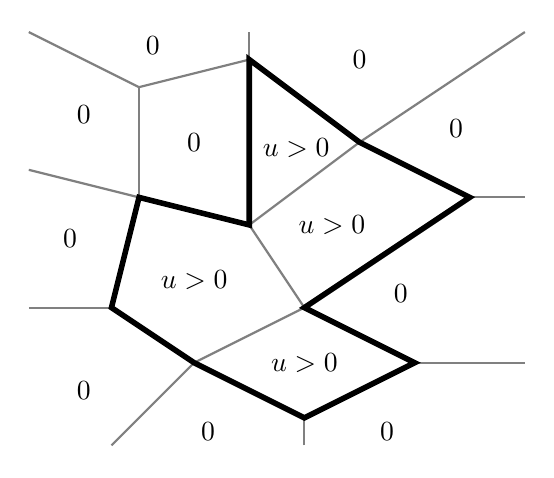
\begin{tikzpicture}[scale=0.35]
  \draw[gray, thick] (3,0) -- (6,3);
  \draw[gray, thick] (0,5) -- (3,5);
  \draw[gray, thick] (0,10) -- (4,9);
  \draw[gray, thick] (0,15) -- (4,13);
  \draw[gray, thick] (4,13) -- (4,9);
  \draw[gray, thick] (4,13) -- (8,14);
  \draw[gray, thick] (8,14) -- (8,15);
  \draw[gray, thick] (12,11) -- (18,15);
  \draw[gray, thick] (10,5) -- (14,3);
  \draw[gray, thick] (10,1) -- (14,3);
  \draw[gray, thick] (14,3) -- (18,3);
  \draw[gray, thick] (6,3) -- (10,1);
  \draw[gray, thick] (6,3) -- (10,5);
  \draw[gray, thick] (10,0) -- (10,1);
  \draw[gray, thick] (10,5) -- (8,8);
  \draw[gray, thick] (8,8) -- (12,11);
  \draw[gray, thick] (16,9) -- (18,9);

  % the free boundary is bold
  \draw[line width=2.0pt] (6,3) -- (3,5) -- (4,9) -- (8,8) -- (8,14) --
                          (12,11) -- (16,9) -- (10,5) -- (14,3) -- (10,1) -- cycle;
  % label cells with positive thickness
  \draw (6,6) node {$u>0$};
  \draw (11,8) node {$u>0$};
  \draw (9.7,10.8) node {$u>0$};
  \draw (10,3) node {$u>0$};
  % label cells with zero thickness
  \draw (2,2) node {$0$};
  \draw (1.5,7.5) node {$0$};
  \draw (2,12) node {$0$};
  \draw (4.5,14.5) node {$0$};
  \draw (6,11) node {$0$};
  \draw (12,14) node {$0$};
  \draw (15.5,11.5) node {$0$};
  \draw (13.5,5.5) node {$0$};
  \draw (13,0.5) node {$0$};
  \draw (6.5,0.5) node {$0$};
\end{tikzpicture}

\end{center}
\caption{The ``boundary leak'' $B_n^h$ is computed along those edges where wet and dry cells meet.}
\label{fig:fvmesh-leak}
\end{figure}

\subsection{Complementarity and cell-wise conservation}  \label{subsec:ncp}  The continuous-space, discrete-time weak formulation we propose in Sections \ref{sec:weakform} and \ref{sec:wellposed}, using variational inequalities (VIs) \eqref{eq:theVI}, would typically be solved using finite element (FE) discretization \cite[for example]{CalvoDuranyVazquez2000,JouvetBueler2012,
JouvetBuelerGraeserKornhuber2013}.  On the other hand we have just applied the FV language of discrete conservation.  These views can be harmonized by observing that a VI is equivalent to a complementarity problem \cite{FacchineiPang2003,KinderlehrerStampacchia1980}.  Practical solver algorithms, and clearer intuition, can result from this observation.  The schemes described next are (simultaneously) $W_0^{1,p}$-conforming and implementable using finite-dimensional complementarity-problem solvers (see below).

Suppose we discretize using an FE subspace $S^h \subset \mathcal{X} = W_0^{1,p}(\Omega)$ of dimension $m$, based on a triangulation (or other mesh) of $\Omega$ with resolution $h$.  Consider problem \eqref{eq:theVI} on this space, namely
\begin{equation}
\ip{A_n(u_n^h)}{v^h-u_n^h} \ge 0 \quad \text{for all } v \in \mathcal{K} \cap S^h,   \label{eq:FEtheVI}
\end{equation}
where $A_n$ is given by \eqref{eq:defineAn} and (as usual) $\mathcal{K} = \{u\in \mathcal{X}\,\big|\,u\ge 0\}$.  Under the same Section \ref{sec:wellposed} hypotheses considered for \eqref{eq:theVI}, we assume problem \eqref{eq:FEtheVI} is well-posed for the numerical solution $u_n^h \in \mathcal{K} \cap S^h$.  Next suppose there is an admissible nodal basis $\{\psi_i\}$ of $S^h$, i.e.~such that $\psi_i(x)\ge 0$ on $\Omega$ and $v(x) = \sum_i v(x_i) \psi_i(x)$ for some nodes $x_i$.  (For example, the usual hat-function bases for $P_1$ and $Q_1$ elements would satisfy this hypothesis, but not the nodal $P_2$ basis \cite{Elmanetal2014}.)  Then we can represent the FE solution $u_n^h$ by a vector $\tilde u \in \RR_+^m$, i.e.~such that $u_i = u_n^h(x_i) \ge 0$.

Up to isomorphism the nonlinear operator in FE formulation \eqref{eq:FEtheVI} is a map $\tilde A:\RR_+^m \to (\RR^m)'$ with entries $\tilde A(\tilde u)^i = \ip{A_n(u_n^h)}{\psi_i} \in \RR$.  The finite-dimensional VI \eqref{eq:FEtheVI} is equivalent to the nonlinear complementarity problem (NCP)
\begin{equation}
\tilde u_i \ge 0, \quad \tilde A(\tilde u)^i \ge 0, \quad \tilde u_i \tilde A(\tilde u)^i = 0 \label{eq:FEtheNCP}
\end{equation}
\cite[Theorem I.5.5]{KinderlehrerStampacchia1980}; see also \cite{FacchineiPang2003}.  The final complementarity condition in \eqref{eq:FEtheNCP} can be regarded either entrywise or as an inner-product because of the nonnegativity of the factors.  Problem \eqref{eq:FEtheNCP} is nonlinear even if the operator $A_n$ is linear, and thus iteration is expected in any numerical solution.  Scalable Newton schemes for NCP problems are described in \cite{BensonMunson2006}; relevant applications appear in \cite{Brinkerhoffetal2017,Bueler2016}.

In our fluid-layer context the intuition behind NCP \eqref{eq:FEtheNCP} is straightforward.  Namely, at convergence of the numerical solver:
\renewcommand{\labelenumi}{(\roman{enumi})}
\begin{enumerate}
\item the layer thickness at each node is nonnegative,
\item the balance between flow and climate inputs, represented by the residual of the operator $A_n$ in the direction of test function $\psi_i$, never removes more mass than was already present, and
\item either the thickness is zero or the flow and climate are in exact balance.
\end{enumerate}

\smallskip
When the value $\tilde A(\tilde u)^i = \ip{A_n(u_n^h)}{\psi_i}$ is zero then mass conservation (balance) equation \eqref{eq:semimassconserve} holds at node $x_i$ in an FE sense.  That is, a weighted-average of the integrand in \eqref{eq:defineAn}, over the support of $\psi_i(x)$, is zero.  Tradition and climate-modeling practice regards such an averaged sense of discrete balance as inferior to exact local balance \eqref{eq:fvlocalconservation}, but one may adapt \eqref{eq:FEtheNCP} to an FV view by assuming that for each FE node $x_i$ there is a unique corresponding FV cell $\omega_i$ (Subsection \ref{subsec:spacenotation}).  The schemes in \cite{Bueler2016,EwingLinLin2002,Ringleretal2013}, for example, satisfy this condition.  Generally such a scheme can be interpreted as having ``dual meshes,'' namely cells for conservation plus a mesh for representing the solution \cite{Ringleretal2013}, but in fact we will need no detailed assumptions about the correspondence in the following computations.

Suppose we compute the residual using the characteristic function of each cell:
\begin{align}
\hat A(\tilde u)^i &= \ip{A_n(u_n^h)}{\mathbbm{1}_{\omega_i}}  \label{eq:cellwiseresidual} \\
                   &= \int_{\omega_i} \left(u_n^h - \Delta t_n F_n^h - u_{n-1}^h\right) + \Delta t_n \sum_{k\in\mathcal{E}_i} \int_{(i,k)} \bQ_n^h\cdot \bn_{(i,k)}. \notag
\end{align}
where $F_n^h = F_n(u_n^h,x)$ and $\bQ_n^h = \bQ_n(\grad u_n^h, u_n^h,x)$.  Regarding the flux calculation we will again assume local balance \eqref{eq:fvlocalconservation} between fluid-filled cells.  The integral $\ip{A_n(u_n^h)}{\mathbbm{1}_{\omega_i}}$ must be understood in a distributional sense, for instance as a limit using mollification of $\mathbbm{1}_{\omega_i}$.  Note that $\mathbbm{1}_{\omega_i} \notin \mathcal{X}$, so this is a Petrov-Galerkin formulation, but the scheme is conforming in the sense that $u_n^h\in \mathcal{K}\cap S^h$ is admissible \cite{Elmanetal2014}.  Such a combined ``finite volume element'' viewpoint is not new as it applies to PDE problems \cite[for example]{Cai1990,EwingLinLin2002}, but it seems not to be widely used for VIs.

The NCP corresponding to the VI for \eqref{eq:cellwiseresidual}, namely
\begin{equation}
\tilde u_i \ge 0, \quad \hat A(\tilde u)^i \ge 0, \quad \tilde u_i \hat A(\tilde u)^i = 0, \label{eq:FVtheNCP}
\end{equation}
again has a clear interpretation even though it mixes FE and FV aspects.  For each cell $\omega_i$ the nodal thickness $\tilde u_i$ is nonnegative, the flow and climate will not remove more mass than was already present in the cell ($\hat A(\tilde u)^i \ge 0$), and either the nodal thickness is zero or conservation (balance) is exact in a cell-wise sense.

However, use of \eqref{eq:cellwiseresidual} and \eqref{eq:FVtheNCP} requires a revised global balance accounting relative to Subsection \ref{subsec:leak}.  We redefine
\begin{equation}
M_n^h = \int_\Omega u_n^h, \quad C_n^h = \Delta t_n \sum_{\tilde u_i>0} \int_{\omega_i} F_n^h, \quad R_n^h = \sum_{\tilde u_i=0} \int_{\omega_i} u_{n-1}^h, \label{eq:newfvtimeseriesdefn}
\end{equation}
to replace \eqref{eq:fvtimeseriesdefn}, and
\begin{equation}
B_n^h = \Delta t_n \sum_{\tilde u_i > 0, \tilde u_k = 0, k\in\mathcal{E}_j} \int_{(i,k)} \bQ_n^h \cdot \bn_{(i,k)} \label{eq:newfvdefineleak}
\end{equation}
to replace \eqref{eq:fvdefineleak}.  Noting that $u_n^h$ may be nonzero on a cell $\omega_i$ corresponding to a zero nodal thickness $\tilde u_i=0$, the following calculation applies if $\tilde u$ solves NCP \eqref{eq:FVtheNCP}:
\begin{align}
M_n^h - M_{n-1}^h &= \sum_{\tilde u_i>0} \int_{\omega_i} u_n^h - u_{n-1}^h + \sum_{\tilde u_i=0} \int_{\omega_i} u_n^h - u_{n-1}^h \label{eq:newfvcalculation} \\
  &= C_n^h - \Delta t_n \sum_{\tilde u_i>0} \sum_{k\in \mathcal{E}_i} \int_{(i,k)} \bQ_n^h \cdot \bn_{(i,k)} + \sum_{\tilde u_i=0} \int_{\omega_i} u_n^h - R_n^h \notag
\end{align}
The flux sum again simplifies through cancellation by local conservation \eqref{eq:fvlocalconservation}, but now we must add a new time series, which we call the \emph{cell slop}, because the support of $u_n^h$ generally extends outside of the wet cells:
\begin{equation}
S_n^h = \sum_{\tilde u_i=0} \int_{\omega_i} u_n^h. \label{eq:fvdefineslop}
\end{equation}

With the revised definitions, by \eqref{eq:newfvcalculation} the following balance holds,
\begin{equation}
  M_n^h = M_{n-1}^h + C_n^h - R_n^h - B_n^h + S_n^h, \label{eq:newfvfinalbalance}
\end{equation}
replacing \eqref{eq:fvfinalbalance} and \eqref{eq:newbalance}.  Time series \eqref{eq:newfvtimeseriesdefn}, \eqref{eq:newfvdefineleak}, and \eqref{eq:fvdefineslop} are computable \emph{a posteriori} although quadrature may be needed depending on the form of functions $F_n$ and $\bQ_n$.  In conclusion, compared to the fixed-boundary balance \eqref{eq:oldbalance}, \eqref{eq:newfvfinalbalance} identifies three conservation errors for free-boundary problems.  The retreat loss $R_n^h\to 0$ under temporal refinement, the boundary leak $B_n^h\to 0$ under spatial refinement, and the cell slop $S_n^h$ is identically zero in a pure FV formulation (Subsection \ref{subsec:leak}).


\section{Conclusion} \label{sec:conclusion}

Global-scale fluid models sometimes claim exact discrete conservation as a goal \cite{Ringleretal2013,Thuburn2008}, but these claims are apparently made in a fixed-boundary context.  On the other hand, multiphysics Earth system models attempt to conserve masses of the phases of water (in particular) separately, as these phases have different physical properties relevant to climate dynamics.  (For example, snow and ice have higher albedo and lower density than the liquid ocean.)  Within such models it is common for one or more fluids or phases to form a thin layer with a moving (free) lateral boundary, a description which applies to ice sheets, glaciers, sea ice, sub-glacial liquid water, and evaporable seas and lakes, among others.  The current paper supposes that discrete mass conservation, up to rounding errror, does not occur in such free-boundary subsystems, though conservation is recoverable in the temporal and spatial refinement limit, and these models sometimes include \emph{ad hoc} redistribution schemes which globally balance the mass-conservation books.  However, conscientious numerical model design suggests quantification of conservation errors, not sweeping them under the refinement-limit or other rugs.

We address the modeling of thin fluid layers through semidiscretization in time (Section \ref{sec:strongform}), and then weak formulation as a sequence of continuous-space VIs (Sections \ref{sec:weakform} and \ref{sec:wellposed}), always based on the fundamental nonnegative thickness condition, but a spatial discretization must, of course, also be used in numerical models.  We interpret discrete mass conservation first through an FV framework (Section \ref{sec:spacediscretized}), and then Subsection \ref{subsec:ncp} reconciles this viewpoint to an FE solution of the VIs.  The actual intent of Section \ref{sec:spacediscretized} is to suggest that modelers do simple conservation arithmetic on the NCP (or VI) form of the problem solved at each time step.

For numerical models we have identified the per time-step retreat set $\Omega_n^r$ (Subsection \ref{subsec:setdecompose}) and retreat mass loss $R_n$ (Section \ref{sec:timeseries}) as fundamental.  The former is the (continuous-space) region where the fluid layer thickness is positive at the beginning of the time step, and, through flow and (climatic) source terms, becomes zero at the end of the step.  Fluid is completely removed in the retreat set at some time during the time step, and, intuitively, the numerical model has no access to the (substep) time and manner in which this occurs, other than in the inequality sense that the climate was sufficiently ablative so as to eliminate the fluid.  Note that the retreat area $|\Omega_n^r|$ can be arbitrarily large even for short time steps.  For example, in a climate model a large area of thin ice sheet or sea ice can melt, or a large area of water on the ground can evaporate.  The retreat loss $R_n$, however, which is a mass, can be bounded \emph{a priori} (Section \ref{sec:timeseries}), though it cannot be exactly balanced by a computable integral of the source term during the time step.

Conclusions which apply in the semi-discretized, continuous-space case are independent of any particular spatial discretization scheme.  However, in Section \ref{sec:spacediscretized} we define computable conservation error quantities at the discretized free boundary.  With these computable time series in hand a numerical solver can balance the books up to rounding error in a manner which properly reflects the model.  Even without \emph{a priori} control of the free boundary, a user can assess whether \emph{a posteriori} conservation errors are acceptably small, and shorten time steps or refine meshes if not.  Climate models, in particular, can thereby have better-controlled uncertainty in mass transfers between component fluids of the Earth system.


%         References
\bibliographystyle{siamplain}
\bibliography{lc}


\appendix

\section{Inequalities for $p$-norms}   \label{app:pinequalities}  Versions of the inequalities in the next two Lemmas appear in the literature, at least as early as \cite{GlowinskiMarroco1975}, but here the results apply in $\RR^d$---contrast \cite{BarrettLiu1993,GlowinskiMarroco1975} for the $\RR^2$ case---and have complete proofs and explicit constants.  The first two proofs follow \cite[Appendix A]{Peral1997}.

\begin{lemma}  \label{lem:pbiginequality}  If $p\ge 2$ and $x,y\in\RR^d$ then
\begin{equation}
\left(|x|^{p-2} x - |y|^{p-2} y\right)\cdot(x-y) \ge 2^{2-p} |x-y|^p. \label{eq:pbiginequality}
\end{equation}
The constant is sharp; consider $y=-x$.
\end{lemma}

\begin{proof}  The case where $x=0$ or $y=0$ is trivial, so assume, by swapping $x$ and $y$ as necessary, that $0 < |y| \le |x|$.  Define $t=|y|/|x|$ and $s = (x\cdot y)/(|x||y|)$ so that $0\le t \le 1$ and $|s|\le 1$.  Expand \eqref{eq:pbiginequality} and divide it by $|x|^p$, to get the equivalent statement
    $$1 - (t^{p-1}+t) s + t^p \ge 2^{2-p} \left(1 - 2 s t + t^2\right)^{p/2}.$$
It is easy to check that this holds when $s=1$, so now we need to prove that $2^{2-p}$ is a lower bound for
	$$f(t,s) = \frac{1 - (t^{p-1}+t) s + t^p}{\left(1 - 2 s t + t^2\right)^{p/2}}.$$
on $(t,s) \in R=[0,1]\times[-1,1)$.  Note $1-2st+t^2 > 0$ on $ R$, so $f(t,s)$ is well-defined and differentiable on $R$.

Now, $f(t,-1) = \left(1 + t^{p-1}\right) / \left(1 + t\right)^{p-1}$ on $t\in[0,1]$.  Because $h(t)=t^{p-1}$ is convex for $p \ge 2$,
    $$\frac{1}{2^{p-1}} (1+t)^{p-1} = h(\tfrac{1}{2} 1 + \tfrac{1}{2} t) \le \tfrac{1}{2} h(1) + \tfrac{1}{2} h(t) = \tfrac{1}{2} (1 + t^{p-1}),$$
and thus $f(t,-1) \ge 2^{2-p}$.  On the other hand, a quick calculation shows
    $$\frac{\partial f}{\partial s} = \frac{t}{\left(1 - 2 s t + t^2\right)^{(p+2)/2}} g(t,s)$$
where
    $$g(t,s) = s(2-p) t (t^{p-2} + 1) + (p-1) (t^p+1) - t^{p-2} - t^2$$
is continuous on the closed rectangle $\bar R = [0,1]\times[-1,1]$.  We will show $g(t,s)\ge 0$ on $\bar R$, thus that $\partial f/\partial s \ge 0$ on $R$, and thus that $f(t,s)\ge f(t,-1) \ge  2^{2-p}$ on $R$.

Now,
    $$\frac{\partial g}{\partial s} = (2-p) t (t^{p-2} + 1) \le 0$$
on $\bar R$.  Define $G(t) = g(t,1)$.  We will show $G(t)\ge 0$ on $[0,1]$, thus that $g(t,s)\ge g(t,1)\ge 0$ on $\bar R$.  But $G(t)\ge 0$ is equivalent to $(p-1) (t-1) (t^{p-1}-1) \ge (t^{p-2} - t) (1 - t)$ which is in turn equivalent to $(p-1) (1 - t^{p-1}) \ge t^{p-2} - t$.  Note $(p-1) (1 - t^{p-1}) \ge 0$.  If $p\ge 3$ then $t^{p-2} - t \le 0$ so $G(t)\ge 0$ in that case.  On the other hand, if $2\le p < 3$ then
	$$\frac{t^{p-2} - t}{1 - t^{p-1}} = t^{p-2} \frac{1 - t^{3-p}}{1 - t^{p-1}} \le t^{p-2} \le 1 \le p-1$$
on $t\in[0,1)$, because $t^{p-1}\le t^{3-p}$ and thus $1 - t^{p-1} \ge 1 - t^{3-p}$.  But also $G(1)=0$, so $G(t)\ge 0$ on $[0,1]$. \end{proof}

\begin{lemma}  \label{lem:psmallinequality}  If $1<p\le 2$ and $x,y\in\RR^n$ then
\begin{equation}
\left(|x|^{p-2} x - |y|^{p-2} y\right)\cdot(x-y) \ge (p-1)\, |x-y|^2 \, \left(|x|+|y|\right)^{p-2}. \label{eq:psmallinequality}
\end{equation}
\end{lemma}

\begin{proof}  Assuming $x,y$ are not both zero, by symmetry (swapping $x$ and $y$) and homogeneity (replacing $x,y$ with $\lambda x,\lambda y$) we can assume $|x| = 1 \ge |y|$.  Furthermore, by choosing a basis of $\RR^d$ we can have $x=(1,0,\dots,0)$ and $y=(y_1,y_2,0,\dots,0)$ where $y_1^2+y_2^2 \le 1$.  In these terms, the inequality we seek to prove is
\begin{align*}
&\left(1 - (y_1^2+y_2^2)^{\frac{p-2}{2}} y_1\right) (1-y_1) + (y_1^2+y_2^2)^{\frac{p-2}{2}} y_2^2 \\
&\qquad\qquad \ge (p-1)\, \left((1-y_1)^2+y_2^2\right) \left(1 + \sqrt{y_1^2+y_2^2} \right)^{p-2}.
\end{align*}
(Compare equation (A.4) in \cite{Peral1997}.)  But
\begin{align*}
1 - (y_1^2+y_2^2)^{\frac{p-2}{2}} y_1
      &\ge \begin{cases} 1-y_1, & y_1 \le 0, \\
                        1-y_1^{p-1}, & 0 \le y_1 \le 1 \end{cases}\Bigg\}
      \ge (p-1) (1-y_1).
\end{align*}
(The lower case in the last inequality is easy to prove by the mean-value-theorem applied to $\varphi(t)=t^{p-1}$, for which $\varphi'(1)=p-1$ is the minimum value of the derivative on $t\in[0,1]$.)  Also noting $(y_1^2+y_2^2)^{\frac{p-2}{2}} \ge 1$ and $\left(1 + \sqrt{y_1^2+y_2^2} \right)^{2-p} \ge 1$, because $|y|\le 1$ and $p-2\le 0$, thus
\begin{align*}
&\frac{\left(1 - (y_1^2+y_2^2)^{\frac{p-2}{2}} y_1\right) (1-y_1) + (y_1^2+y_2^2)^{\frac{p-2}{2}} y_2^2}
      {\left((1-y_1)^2+y_2^2\right) \left(1 + \sqrt{y_1^2+y_2^2} \right)^{p-2}} \\
&\qquad \ge \frac{(p-1) (1-y_1)^2 + y_2^2}
      {(1-y_1)^2+y_2^2} \,  \left(1 + \sqrt{y_1^2+y_2^2} \right)^{2-p} \\
&\qquad \ge \frac{(p-1) (1-y_1)^2 + (p-1) y_2^2}{(1-y_1)^2+y_2^2} = p-1.
\end{align*}
This proves \eqref{eq:psmallinequality}. \end{proof}

We will also need the result of combining point-wise Lemma \ref{lem:psmallinequality} with integration over a set $\Omega$.

\begin{lemma} \label{lem:smallpbound}  Suppose $1<p\le 2$.  If $\Omega \subset \RR^d$ is measurable and if $\bu,\bv\in L^p(\Omega; \RR^m)$ for $m\ge 1$, then
\begin{equation}
    \int_\Omega \frac{|\bu-\bv|^p}{\left(|\bu|+|\bv|\right)^{2-p}} \ge \frac{\|\bu-\bv\|_{L^p(\Omega; \RR^m)}^2}{\big\||\bu|+|\bv|\big\|_{L^p(\Omega)}^{2-p}}. \label{eq:smallpbound}
\end{equation}
\end{lemma}

\begin{proof}  By H\"older inequality with $r=2/p$ and $s=2/(2-p)$, so $r^{-1}+s^{-1}=1$,
\begin{align*}
\int_\Omega |\bu - \bv|^p &= \int_\Omega \frac{|\bu-\bv|^p}{\left(|\bu|+|\bv|\right)^{p(2-p)/2}} \left(|\bu|+|\bv|\right)^{p(2-p)/2} \\
    &\le \left(\int_\Omega \frac{|\bu-\bv|^2}{\left(|\bu|+|\bv|\right)^{2-p}}\right)^{p/2} \left(\int_\Omega \left(|\bu|+|\bv|\right)^p\right)^{(2-p)/2},
\end{align*}
thus \eqref{eq:smallpbound}.
\end{proof}

Finally we recall the Poincar\'e inequality on the Sobolev space $W_0^{1,p}(\Omega)$.  This form, with an explicit but not optimal constant, is from \cite[section 7.8]{GilbargTrudinger2001}.

\begin{lemma} \label{lem:poincare}  If $\Omega\subset \RR^d$ is a bounded domain with volume $|\Omega|$, and if $1\le p<\infty$ then for all $u\in W_0^{1,p}(\Omega)$,
\begin{equation}
  \|u\|_{W^{1,p}(\Omega)}^p \le C(\Omega,p) \int_\Omega |\grad u|^p, \label{eq:poincare}
\end{equation}
where $C(\Omega,p)=1+(|\Omega|/\omega_d)^{p/d}$ and $\omega_d=(2 \pi^{d/2})/(d\,\Gamma(d/2))$ is the volume of the unit ball in $\RR^d$.
\end{lemma}


\section{Second-order Runge-Kutta time-discretization}  \label{app:rk2}  Section \ref{sec:strongform} describes the time semi-discretization of the continuum strong form \eqref{eq:massconserve}--\eqref{eq:constraint} using the $\theta$ method.  Such a one-stage method generates particular forms for the functions $\bQ_n(\bX,v,z)$ and $F_n(v,z)$ in equations \eqref{eq:semimassconserve}--\eqref{eq:semiconstraint}, and these functions then define weak formulation (VI) \eqref{eq:theVI}.  Here we illustrate how the corresponding functions $\bQ_n$ and $F_n$ can be generated for second-order Runge-Kutta (RK) schemes.

For the $m$-dimensional ODE system $\by' = \bg(t,\by)$ an $s$-stage RK scheme \cite{AscherPetzold1998} with time-step $h=\Delta t$ is given by constants $a_{ij},b_i,\tau_i$ and the equations
\begin{align}
  \by_{n,i} &= \by_{n-1} + h \sum_{j=1}^s a_{ij} \bg(t_{n-1} + \tau_j h, \by_{n,j}), \quad i=1,\dots,s \label{eq:RK2} \\
      \by_n &= \by_{n-1} + h \sum_{i=1}^s b_i \bg(t_{n-1} + \tau_i h, \by_{n,i}). \notag
\end{align}
\emph{Explicit} methods have $a_{ij}=0$ for $j\ge i$, i.e.~zeros on and above the diagonal in the Butcher tableau \cite{AscherPetzold1998}, while \emph{semi-implicit} methods have zeros above the diagonal.  Whereas general implicit RK schemes generate larger (nonlinear) systems, semi-implicit methods have the computational advantage that each stage generates an $m$-equation system.  Note that one must solve \eqref{eq:theVI} $s$ times to compute a time step using an $s$-stage explicit or semi-implicit RK scheme.

\emph{Diagonally-implicit} RK (DIRK) methods are semi-implicit methods for which the diagonal entries $a_{ii}$ are independent of $i$.  The accuracy of $s$-stage DIRK methods is limited to order $p=s+1$, and there exist strongly S-stable and stiffly-accurate \cite{AscherPetzold1998} DIRKs with order $p=s$ for $s=1,2,3$ \cite{Alexander1977}.  (``Strongly S-stable'' is also called ``stiff decay'' \cite{AscherPetzold1998}.)  The stability properties of these DIRK methods are helpful for mass conservation problems considered in the text, especially cases where $\bq$ has a leading-order diffusion term so that the $m$-dimensional method-of-lines ODE system is stiff.  In DIRK methods the linear system matrix can potentially be re-used at each stage.  (This matrix is $A = I - h a_{ii} J$ where the Jacobian $J$ is evaluated at the start of the time step, $J = \frac{\partial \bg}{\partial y}(t_{n-1},\by_{n-1})$.)

Now, as an illustration, we compute functions $\bQ_n$ and $F_n$ for two DIRK schemes.

\medskip
\renewcommand{\labelenumi}{\emph{(\alph{enumi})}}
\begin{enumerate}
\item The implicit midpoint rule is a $(s,p)=(2,2)$ A-stable DIRK scheme.  It uses a half backward Euler step followed by an explicit step:
\begin{align}
\tilde\by &= \by_{n-1} + \tfrac{1}{2} h \bg(t_{n-1}+\tfrac{1}{2}h,\tilde\by), \notag \\
\by_n &= \by_{n-1} + h \bg(t_{n-1}+\tfrac{1}{2}h,\tilde\by). \notag
\end{align}
Let $t_{n-1/2} = t_{n-1} + \tfrac{1}{2} \Delta t$.  Functions \eqref{eq:functionalforms} for the first stage are
  $$\tilde\bQ(\bX,v,x) = \tfrac{1}{2} \bq(\bX,v,x,t_{n-1/2}) \quad \text{and} \quad \tilde F(v,x) = \tfrac{1}{2} f(v,x,t_{n-1/2}).$$
Now let $\tilde u$ denote the weak solution to the first stage VI problem.  The functions for the explicit second stage are then $\bQ_n(\bX,v,x) = 0$ and
  $$\quad F_n(v,x) = f(\tilde u,x,t_{n-1/2}) - \Div \bq(\grad\tilde u,\tilde u,x,t_{n-1/2}).$$

\item The (unique) strongly S-stable $(s,p)=(2,2)$ scheme for which $0\le \tau_i\le 1$ \cite{AscherPetzold1998} has equations
\begin{align}
\tilde\by &= \by_{n-1} + \alpha h \bg(\tilde t,\tilde\by), \notag \\
\by_n &= \by_{n-1} + (1-\alpha) h \bg(\tilde t,\tilde\by) + \alpha h \bg(t_n,\by_n). \notag
\end{align}
where $\alpha = 1-\frac{\sqrt{2}}{2}$ and $\tilde t = t_{n-1} + \alpha h$.  Functions for the first stage are
  $$\tilde\bQ(\bX,v,x) = \alpha \bq(\bX,v,x,\tilde t) \quad \text{and} \quad \tilde F(v,x) = \alpha f(v,x,\tilde t).$$
If $\tilde u$ denotes the solution to the first stage VI then the functions for the second stage are $\bQ_n(\bX,v,x) = \alpha \bq(\bX,v,x,t_n)$ and
   $$F_n(v,x) = (1-\alpha) f(\tilde u,x,\tilde t) + \alpha f(v,x,t_n) - (1-\alpha) \Div \bq(\grad\tilde u,\tilde u,x,\tilde t).$$
\end{enumerate}

\end{document}
